\documentclass[a4paper]{article}
\usepackage[utf8x]{inputenc}
\usepackage[colorlinks=true, citecolor = green,urlcolor=blue, filecolor = blue]{hyperref}
\usepackage{setspace, amsmath, amsfonts, amssymb, amsthm, enumerate, color, graphicx, verbatim}
\usepackage[left=1in, right=1.0in, top=1.0in, bottom=1.0in]{geometry}
\usepackage{multirow}
\usepackage[T2A]{fontenc} 
\usepackage[serbianc]{babel}
\usepackage{listings}
\usepackage{caption}
\usepackage{subcaption}
\definecolor{mygreen}{RGB}{28,172,0} % color values Red, Green, Blue
\definecolor{mylilas}{RGB}{170,55,241}

\newcommand{\HRule}{\rule{\linewidth}{0.5mm}}
\newcommand{\conj}{\overline}
\newcommand{\trig}{r(\cos\varphi+i\sin\varphi)}	
\newcommand{\trign}{r^n(\cos(n\varphi)+i\sin(n\varphi))}
\newcommand{\trigj}{r(\cos\alpha+i\sin\alpha)}
\renewcommand{\vec}{\overrightarrow}


\begin{document}

\lstset{language=Matlab,%
    %basicstyle=\color{red},
    breaklines=true,%
    morekeywords={matlab2tikz},
    keywordstyle=\color{blue},%
    morekeywords=[2]{1}, keywordstyle=[2]{\color{black}},
    identifierstyle=\color{black},%
    stringstyle=\color{mylilas},
    commentstyle=\color{mygreen},%
    showstringspaces=false,%without this there will be a symbol in the places where there is a space
    numbers=left,%
    numberstyle={\tiny \color{black}},% size of the numbers
    numbersep=9pt, % this defines how far the numbers are from the text
    emph=[1]{for,end,break},emphstyle=[1]\color{red}, %some words to emphasise
    %emph=[2]{word1,word2}, emphstyle=[2]{style},    
}


\begin{titlepage}

\begin{center}


% Upper part of the page   

\textsc{\Huge \textbf{Електротехнички факултет}}\\[5cm]

\textsc{\Huge \textbf{Извештај домаћег}}\\[0.5cm]
\textsc{\large{\textbf{из препознавања облика}}}
\\[4cm]

% Title
\HRule \\[0.8cm]
{ \Huge \bfseries Сви домаћи}\\[0.4cm]

\HRule \\[5cm]

% Author and supervisor
\begin{minipage}{0.55\textwidth}
\begin{flushleft} \large
\emph{Аутор}\\
Ђорђе Живановић, 3013/2017\\
\end{flushleft}
\end{minipage}
\begin{minipage}{0.4\textwidth}
\begin{flushright} \large
\emph{Ментор} \\
Професор Др Жељко Ђуровић
\end{flushright}
\end{minipage}



\vfill

% Bottom of the page
{\large \today}

\end{center}

\end{titlepage}
\tableofcontents
\newpage



\section{Први домаћи задатак}
За руком писаних цифара 6, 8 и 9 која је доступна на сајту предмета испројектовати иновативни систем за препознавање цифара заснован на тестирању хипотеза. Резултате приказати у облику матрице конфузија. Извештај треба да садржи кратки опис испројектованог система, образложени избор обележја као и карактеристичне примере правилно и неправилно класификованих цифара
\subsection{Опис система}
На располагању налазило се 360 руком писаних цифара које су достављене у .bmp формату. Било је по 120 цифара 6, 8 и 9. Задатак је одрађен у програмском пакету \emph{Matlab vR2017b}.  Слике су обрађене у неколико фаза. 
	У првој фази одрађено је бинаризовање слике, тј. вредност свим пикселима је преведена да буде 255 или 0, с обзиром да је слика представљена као низ црних и белих пиксела различитих јачина. Бинаризација је одрађена функцијом \ref{fun:binarize}.
	
	

\renewcommand{\lstlistingname}{Одсечак кода}%
	
\begin{lstlisting}[caption={Бинаризација слике},label={fun:binarize}]
function [binImage] = binarizeImage(image, ratio)
    val = 255 - double(image);
    val(val < ratio * max(max(val))) = 0;
    val(val >= ratio * max(max(val))) = 255;
    binImage = uint8(255 - val);
end

\end{lstlisting}

\noindent Функција прима \emph{image} и \emph{ratio} који представљају дату слику, односно праг бељења-колика црнина се прихвата као белина.  
\\ \indent Друга фаза омогућава одсецање неискоришћеног простора, односно белина. Поред белина занемарене су све мрље унутар белина. Кад се каже мрља мисли се тачка величине бар 5 пиксела (в. сл. \ref{pic:dot6}, \ref{pic:dot8}, \ref{pic:dot9} као пример). 
\begin{figure}[htb!]\caption{Тачке}
\begin{subfigure}{.3\textwidth}
\centering
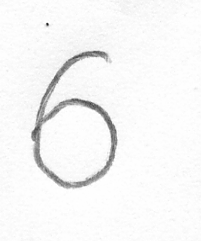
\includegraphics[width=.4\linewidth]{pictures/1/Dot6}
\caption{Тачка у 6}\label{pic:dot6}
\end{subfigure}
\begin{subfigure}{.3\textwidth}
\centering
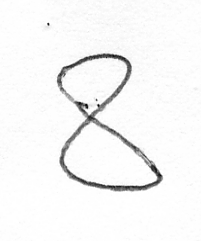
\includegraphics[width=.4\linewidth]{pictures/1/Dot8}
\caption{Тачка у 8}\label{pic:dot8}
\end{subfigure}
\begin{subfigure}{.3\textwidth}
\centering
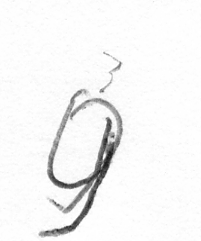
\includegraphics[width=.4\linewidth]{pictures/1/Dot9}
\caption{Тачка у 9}\label{pic:dot9}
\end{subfigure}
\end{figure}

Код за уклањање белина и тачки је одрађен функцијом \ref{fun:cropImage}.

\begin{lstlisting}[caption={Одсецање слике},label={fun:cropImage}]
function [X] = cropImage(image)
    ratio = 0.20;
    X = binarizeImage(image, ratio);
    
    [numRow, numCol] = size(X);
    begin = 1;
    while (begin < numRow) && (sum(X(begin, 1 : numCol)) / numCol > 250 ||...
            sum(X(begin + 1, 1 : numCol)) / numCol > 250 ||...
            sum(X(begin + 2, 1 : numCol)) / numCol > 250 ||...
            sum(X(begin + 3, 1 : numCol)) / numCol > 250 ||...
            sum(X(begin + 4, 1 : numCol)) / numCol > 250 ||...
            sum(X(begin + 5, 1 : numCol)) / numCol > 250)
        begin = begin + 1;
    end

    endV = numRow;
    while(endV > begin)&&...
            (sum(X(endV, 1 : numCol)) / numCol > 250 ||...
            sum(X(endV - 1, 1 : numCol)) / numCol > 250 ||...
            sum(X(endV - 2, 1 : numCol)) / numCol > 250 ||...
            sum(X(endV - 3, 1 : numCol)) / numCol > 250 ||...
            sum(X(endV - 4, 1 : numCol)) / numCol > 250 ||...
            sum(X(endV - 5, 1 : numCol)) / numCol > 250)
        endV = endV - 1;
    end

    left = 1;
    while (left < numCol)&&...
            (sum(X(1 : numRow, left)) / numRow > 250 ||...
            sum(X(1 : numRow, left + 1)) / numRow > 250 ||...
            sum(X(1 : numRow, left + 2)) / numRow > 250 ||...
            sum(X(1 : numRow, left + 3)) / numRow > 250 ||...
            sum(X(1 : numRow, left + 4)) / numRow > 250 ||...
            sum(X(1 : numRow, left + 5)) / numRow > 250)
        left = left + 1;
    end

    right = numCol;
    while (right>1)&&...
            (sum(X(1 : numRow,right)) / numRow > 250 ||...
            sum(X(1 : numRow, right - 1)) / numRow > 250 ||...
            sum(X(1 : numRow, right - 2)) / numRow > 250 ||...
            sum(X(1 : numRow, right - 3)) / numRow > 250 ||...
            sum(X(1 : numRow, right - 4)) / numRow > 250 ||...
            sum(X(1 : numRow, right - 5)) / numRow > 250)
        right = right - 1;
    end

    X = X(begin : endV, left : right);
end

\end{lstlisting}

Овде је коришћен $ratio= 0, 2$  јер даје најбољу тачност за одговарајући скуп података. Међутим и поред свега дође до лошег одсецања (в. сл. \ref{pic:badCrop6}, \ref{pic:badCrop8}).
\begin{figure}[htb!]
\caption{Лоше одсецање}
\begin{subfigure}{.5\textwidth}
\centering

\includegraphics[width=.5\linewidth]{pictures/1/BadCrop6}
\caption{Лоше одсецање 6}\label{pic:badCrop6}
\end{subfigure}
\begin{subfigure}{.5\textwidth}
\centering

\includegraphics[width=.3\linewidth]{pictures/1/BadCrop8}
\caption{Лоше одсецање 8}\label{pic:badCrop8}
\end{subfigure}
\end{figure}

У осталим исправним случајевима добију се бројеви као на сл.  \ref{pic:goodCrop6}, \ref{pic:goodCrop8}, \ref{pic:goodCrop9}.
\begin{figure}[htb!]\caption{Добро одсечене}
\begin{subfigure}{.3\textwidth}
\centering

\includegraphics[width=.4\linewidth]{pictures/1/GoodCrop6}
\caption{Добро одсечена цифра 6}\label{pic:goodCrop6}
\end{subfigure}
\begin{subfigure}{.26\textwidth}
\centering

\includegraphics[width=.4\linewidth]{pictures/1/GoodCrop8}
\caption{Добро одсечена цифра 8}\label{pic:goodCrop8}
\end{subfigure}
\begin{subfigure}{.3\textwidth}
\centering

\includegraphics[width=.48\linewidth]{pictures/1/GoodCrop9}
\caption{Добро одсечена цифра 9}\label{pic:goodCrop9}
\end{subfigure}
\end{figure}

Крајња, трећа фаза рачуна "центар масе" цифара добијених из друге фазе и формира функцију густине расподеле вероватноће за сваку од центара масе цифара 6, 8, 9. Центар маса се рачуна функцијом \ref{fun:calculateCenter}. Функција помера координатни почетак слике тако да буде у центру слике и онда сабира све вредности пиксела померене са одговарајућим вектором положаја. На крају се добијена вредност подели са бројем пискела на слици и то је центар масе дате слике.

\begin{lstlisting}[caption={Центар масе},label={fun:calculateCenter}]
function [center] = calculateCenter(X)
    [numRow, numCol] = size(X);
    centerX = 0;
    centerY = 0;
    for row = 1 : numRow
        for col = 1 : numCol
           val = floor(double(X(row, col)));
           centerX = centerX + val * (row - floor(numRow / 2));
           centerY = centerY + val * (col - floor(numCol / 2));
        end
    end
    center = [centerX; centerY] / (numRow * numCol);
end
\end{lstlisting}

Oбрада цифара за све 3 фазе одрађена је кодом \ref{piece:train}. Овде се може приметити да је узето 300 од 360 слика за тренирање, а 60 за проверу, што је $83\%-17\% $ однос у подели скупа на обучавајући и тренирајући скуп. 

\begin{lstlisting}[caption={Обрада цифара},label={piece:train}]
N = 100;
for i = 1 : N
    name = ['BazaCifara6/baza6' num2str(i, '%03d')];
    X = imread(name, 'bmp');    
    nameCropped = ['BazaCifaraCropped6/baza6' num2str(i, '%03d') '.bmp'];
    croppedImage = cropImage(X);
    imwrite(croppedImage, nameCropped, 'bmp');
    features6(:, i) = calculateCenter(croppedImage);
    
    name = ['BazaCifara8/baza8' num2str(i, '%03d')];
    X = imread(name, 'bmp');  
    nameCropped = ['BazaCifaraCropped8/baza8' num2str(i, '%03d') '.bmp'];
    croppedImage = cropImage(X);
    imwrite(croppedImage, nameCropped, 'bmp');
    features8(:, i) = calculateCenter(croppedImage);
    
    name = ['BazaCifara9/baza9' num2str(i, '%03d')];
    X = imread(name, 'bmp');  
    nameCropped = ['BazaCifaraCropped9/baza9' num2str(i, '%03d') '.bmp'];
    croppedImage = cropImage(X);
    imwrite(croppedImage, nameCropped, 'bmp');
    features9(:, i) = calculateCenter(croppedImage);
end

figure;
hold on
plot(features6(1, :), features6(2, :), 'sb');
plot(features8(1, :), features8(2, :), 'hg');
plot(features9(1, :), features9(2, :), 'ro');
legend('Sest', 'Osam', 'Devet');
title('Skup za obucavanje');
\end{lstlisting}

Приказ расподеле скупа тренирајућих цифара je приказано на слици \ref{fig:Train}.

\begin{figure}[htb!]

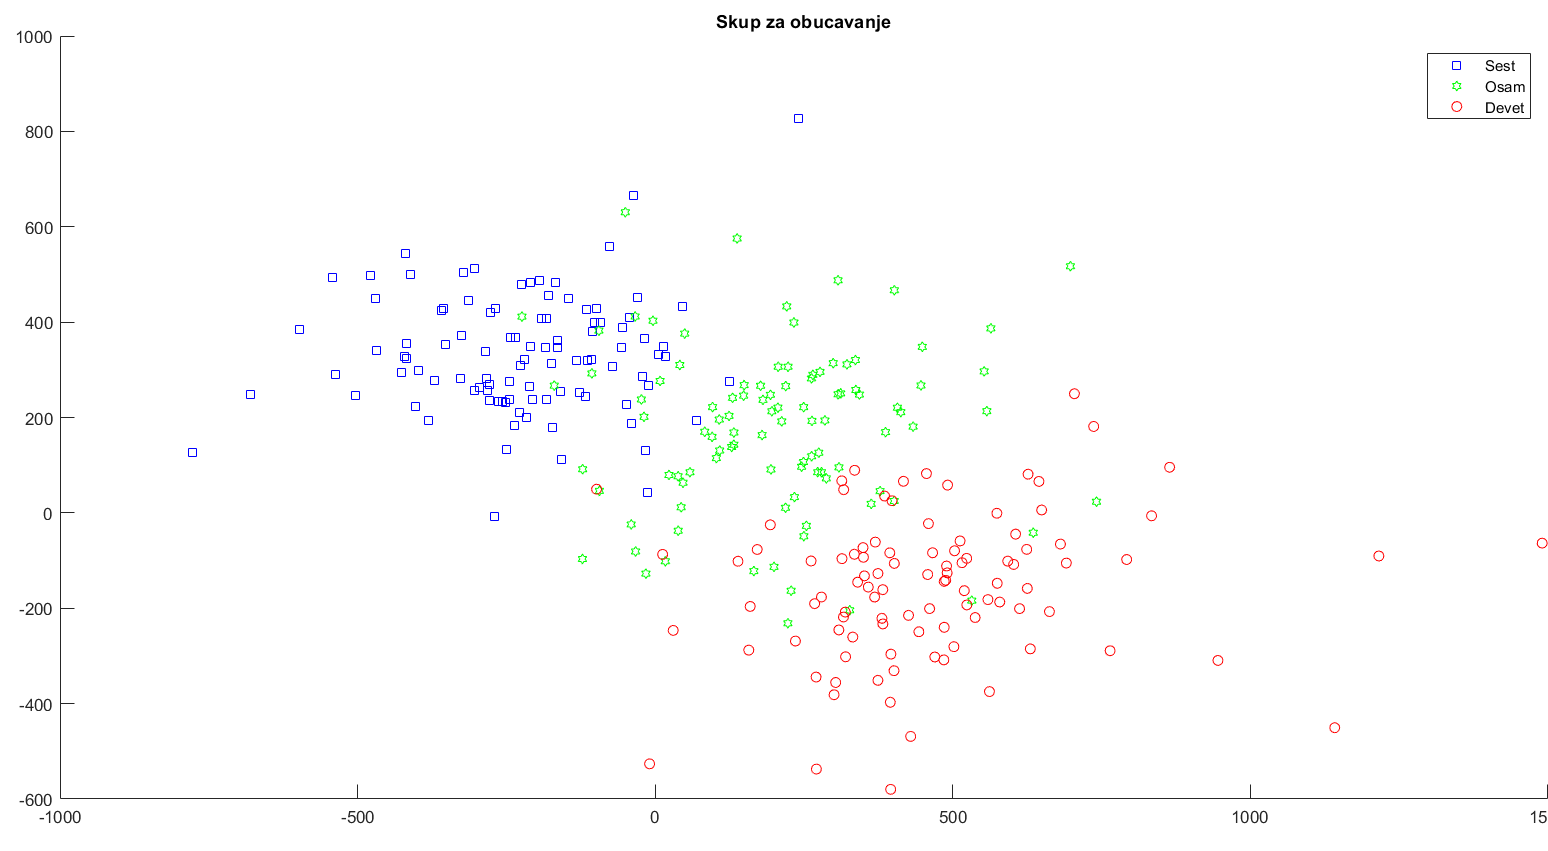
\includegraphics[scale=.42]{pictures/1/TrainSet}
\caption{Oбучавајући скуп}\label{fig:Train}
\end{figure}



Функција густине вероватноће за сваку цифру се рачуна тако што се израчунају математичка очекивања и варијансе за сваки од 3 скупа цифара (в. одсечак \ref{fun:calcExpVar}).

\begin{lstlisting}[caption={Варијансе и математичка очекивања},label={fun:calcExpVar}]
M1 = mean(features6')'; 
S1 = cov(features6');
M2 = mean(features8')'; 
S2 = cov(features8');
M3 = mean(features9')'; 
S3 = cov(features9');
\end{lstlisting}

И потом се израчунају 3 функције густине вероватноће за сваку цифру при чему се густина рачуна користећи функцију \ref{fun:gaus}, при чему се проследе одговарајућа математичка очекивања и коваријациона матрица.
\begin{lstlisting}[caption={Гаусова расподела},label={fun:gaus}]
function [Y] = gausianMultivariate(X, Mx, Sx)
n = size(Sx, 1);
Y = (1 / ((2 * pi) ^(n / 2)  * sqrt(det(Sx)))) * exp((X - Mx)' * inv(Sx) * (X - Mx) / -2);
end
\end{lstlisting}

У зависности која функција густине вероватноће је већа, тој класи припада цифра која се препознаје. Код за одлучивање којој класи припада је дат одсечком \ref{fun:test}.
\begin{lstlisting}[caption={Одлучивање припадности класи},label={fun:test}]
for k = 1:3
    if k == 1
        T = featuresTest6;
    elseif k == 2
        T = featuresTest8;
    else
        T = featuresTest9;
    end
    
    for i = 1 : size(T, 2)
        f1 = gausianMultivariate(T(:, i), M1, S1);
        f2 = gausianMultivariate(T(:, i), M2, S2);
        f3 = gausianMultivariate(T(:, i), M3, S3);
        if (f1 > f2) && (f1 > f3)
            CM(1, k) = CM(1, k) + 1;
            if (k ~= 1)
                fprintf("Predicted: 1 Actual: %d %d\n", k, i + N);
            end
        elseif f2 > f1 && f2 > f3
            CM(2, k) = CM(2, k) + 1;
            if (k ~= 2)
                fprintf("Predicted: 2 Actual: %d %d\n", k, i + N);
            end
        elseif f3 > f2 && f3 > f1
            CM(3, k) = CM(3, k) + 1;
            if (k ~= 3)
                fprintf("Predicted: 3 Actual: %d %d\n", k, i + N);
            end
        end
    end
end

\end{lstlisting}
Добијена матрица конфузије је у табели \ref{tab:matConf}.Можемо да приметимо да је $88,33$ прецизност оваквог препознавања. Такође можемо да приметимо да се 8 најчешће погрешно класификује (4 пута, а 6 и 9 збирно 3 пута су погрешно класификоване), што је за очекивати.
\begin{table}[h!] 
\centering
\caption{Матрица конфузије}\label{tab:matConf}
\vspace*{4mm}
\begin{tabular}{cc|c|c|c|l}
	\cline{3-5}
	& & \multicolumn{3}{ c| }{Стварно} \\ \cline{3-5}
	& & \textit{6} & \textit{8} & \textit{9}  \\ \cline{1-5}
	\multicolumn{1}{ |c  }{\multirow{3}{*}{Класификовано} } &
	\multicolumn{1}{ |c| }{\textit{6}}  & 18 & 3 & 0 &     \\ \cline{2-5}
	\multicolumn{1}{ |c  }{}                        &
	\multicolumn{1}{ |c| }{\textit{8}}  & 2 & 16 & 1 &     \\ \cline{2-5}
	\multicolumn{1}{ |c  }{}                        &
	\multicolumn{1}{ |c| }{\textit{9}}  & 0 & 1 & 19 &     \\ \cline{1-5}
\end{tabular}
\end{table}

\subsection{Избор обележја}
Избор "центра масе" као обележја за које ће се посматрати функција расподеле је разуман јер ако би се 6, 8, 9 и посматрали као објекти, могло би се приметити да је маса 6 пребачена у доњи део, док је за 8 у средњем, а за 9 у горњем, што се може приметити и на слици \ref{fig:Train} јер осмице су груписане око координатног центра, деветке су груписане у горњем делу (негативно за $y$ због тога што за слике је координатни систем обрнут код $y$) и шестице су груписане у доњем делу. Занимљиво је да ће груписање по $x$ оси за шестице и деветке бити симетрично у односу на координатни почетак, јер маса девет је углавном у "десном" крај, а шест у "левом" крају слике. 
\newpage
\subsection{Пример класификација}

\begin{figure}[htb!]\caption{Правилна класификација}
\begin{subfigure}{.3\textwidth}
\centering

\includegraphics[width=.4\linewidth]{pictures/1/GoodClass6}
\caption{Тачка у 6}\label{pic:goodClass6}
\end{subfigure}
\begin{subfigure}{.3\textwidth}
\centering

\includegraphics[width=.4\linewidth]{pictures/1/GoodClass8}
\caption{Тачка у 8}\label{pic:goodClass8}
\end{subfigure}
\begin{subfigure}{.3\textwidth}
\centering

\includegraphics[width=.4\linewidth]{pictures/1/GoodClass9}
\caption{Тачка у 9}\label{pic:goodClass9}
\end{subfigure}
\end{figure}


\begin{figure}[htb!]\caption{Неправилна класификација}
\begin{subfigure}{.3\textwidth}
\centering

\includegraphics[width=.4\linewidth]{pictures/1/BadClass6}
\caption{Класификована 8, а 6 је}\label{pic:goodClass6}
\end{subfigure}
\begin{subfigure}{.3\textwidth}
\centering

\includegraphics[width=.4\linewidth]{pictures/1/BadClass8}
\caption{Класификована 6, а 8 је}\label{pic:goodClass8}
\end{subfigure}
\begin{subfigure}{.3\textwidth}
\centering

\includegraphics[width=.4\linewidth]{pictures/1/BadClass9}
\caption{Класификована 8, а 9 је}\label{pic:goodClass9}
\end{subfigure}
\end{figure}













\newpage
\section{Други домаћи задатак}
По угледу на пример 4.3 из документа Предавање 2, генерисати по $N=500$ одбирака из двеју дводимензионалних класа.
\begin{enumerate}[a)]
\item На дијаграму приказати одбирке
\item Генерисати геометријско место тачака са константном вредношћу функција густина вероватноће па их приказати на дијаграму у простору облика.
\item Испројектовати Бајесов класификатор минималне грешке и на дијаграму, заједно са одбирцима, скицирати класификациону линију, па проценити вероватноћу грешке.
\item Поновити претходну тачку за неки други класификатор по избору.
\item а класе облика генерисаних у претходним тачкама, испројектовати Валдов секвенцијални тест, па скицирати зависност броја потребних одбирака од усвојене вероватноће грешке првог, односно другог типа.
\end{enumerate}

\subsection{Генерисање одбирака}

За почетак генерисаћемо одбирке двеју дводимензионалних класа чије су функције густине вероватноће у облику бимодалних гаусовских расподела:


$$f_1(X) = P_{11} N(M_{11}, \Sigma_{11}) + P_{12} N(M_{12}, \Sigma_{12})$$
$$f_2(X) = P_{21} N(M_{21}, \Sigma_{21}) + P_{22} N(M_{22}, \Sigma_{22}),$$
при чему вероватноће, средње вредности и коваријационе матрице имају следеће вредности:
$$P_{11} = 0,6,  M_{11} = \begin{bmatrix}
   -1,5\\
   4,5
\end{bmatrix}, 
S_{11} = \begin{bmatrix}
				   3,5 & -1\\
				   -1 & 2,2
				\end{bmatrix},
P_{12} = 0,4,  M_{12} = \begin{bmatrix}
										   -0,5\\
										   0,5
										\end{bmatrix}, 
S_{12} = \begin{bmatrix}
				   1,3 & 0,9\\
			   	0,9 &  2
				\end{bmatrix}
$$				
$$P_{21} = 0,45,  M_{21} = \begin{bmatrix}
   7,5\\
   -3,5
\end{bmatrix}, 
S_{21} = \begin{bmatrix}
				   1,5 & 1,1\\
				   1,1 & 1,5
				\end{bmatrix},
P_{22} = 0,55,  M_{22} = \begin{bmatrix}
										   4\\
										   2
										\end{bmatrix}, 
S_{22} = \begin{bmatrix}
				   3 & -0,8\\
			   	-0,8 &  3
				\end{bmatrix}
$$

За генерисање одбирака коришћене су две функције. Одсечак кода прве функције која је коришћена је дат на одсечку \ref{fun:gausGenerate}. Овде се користи својство да се "обична" Гаусова расподела са варијансама 1 и очекивањем 0 кад се помножи са $\Phi \Lambda^\frac{1}{2}$, при чему су $\Phi$ матрица вектора сопствених вредности и $\Lambda$ матрица сопствених вредности од $S_x$, и на крају дода $M_x$, при чему је $M_x$ математичко очекивање вектора за који хоће да се генерише дата расподела, добије се Гаусова расподела са математичким очекивањем $M_x$ и $S_x$.

\renewcommand{\lstlistingname}{Одсечак кода}%
	
\begin{lstlisting}[caption={Вишеваријабална Гаусова расподела-генерисање},label={fun:gausGenerate}]
function [X] = gausianMultivariateGenerate(Mx, Sx, num_points)
% Generates a matrix whose size is num_points, also it has 
% gausian multivarate distribution with Mx mean and 
% Sx covariance matrix. 

[F, L] = eig(Sx);

n = size(Sx, 1);
X = randn(n, num_points);

for i = 1 : num_points
    X(1:n, i) = F * sqrt(L) * X(1:n, i) + Mx; 
end

end
\end{lstlisting}

Друга коришћена функција је дата у одсечку  \ref{fun:gausGenerateModal}. Она користи својство да је бимодална Гаусова расподела збир две Гаусове са одређеним вероватноћама и тако генерише потребну расподелу. 

\begin{lstlisting}[caption={Вишеваријабална мултимодална Гаусова расподела-генерисање},label={fun:gausGenerateModal}]
function [X] = gausianMultimodalGenerate(P1,P2, M1, M2, S1, S2, num_points)
X = zeros(num_points, 2);
for i = 1 : num_points
    probability = rand(1, 1);
    if (probability < P1)
        X(i, :) = gausianMultivariateGenerate(M1, S1, 1);
    else
        X(i, :) = gausianMultivariateGenerate(M2, S2, 1);
    end
end
end
\end{lstlisting}
Позивањем \emph{gausianMultimodalGenerate} са одговарајућим параметрима за обе класе добија се расподела као на слици \ref{fig:Odbirci}. 
\begin{figure}[htb!]
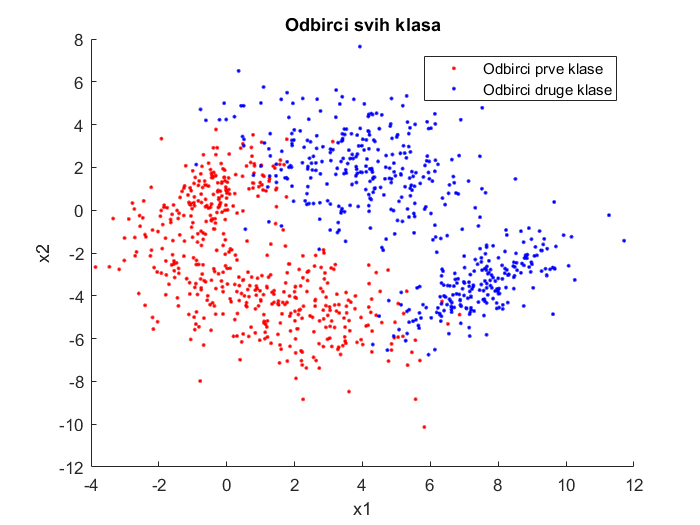
\includegraphics[scale=1]{pictures/2/Odbirci}
\caption{Одбирци}\label{fig:Odbirci}
\end{figure}

\newpage
\subsection{Функција густине вероватноће}
Функција густине вероватноће је израчуната за сваки "део" тако што је за сваку тачку у размаку од $0,1$ у интервалу $[-6, -12]$ на $x$ оси и на интервалу $[-10, 8]$ на $y$ оси позивана функција која је дата одсечком кода \ref{fun:gausMultiModal}. Дата функција густине вероватноће може да се види у \emph{3D} на слици \ref{fig:FGV}. На слици \ref{fig:FGVContour} налазе се геометријска места тачака функције густине вероватноће од сваке класа, и то $0,8 * max(f(X))$, $0,6 * max(f(X))$, $0,4 * max(f(X))$, $0,2 * max(f(X))$. Може да се примети да они делови "класа" који су "оштрији" имају неке вредности које "тупљи" делови немају.

\begin{lstlisting}[caption={Вишеваријабална мултимодална Гаусова расподела-функција густине},label={fun:gausMultiModal}]
function [f] = gausianMultimodal(X, P1, P2, M1, M2, S1, S2)
%GAUSIANMULTIMODAL Calculates multimodal probability density function.
f = P1 * gausianMultivariate(X, M1, S1) + P2 * gausianMultivariate(X, M2, S2); 
end
\end{lstlisting}

\begin{figure}[htb!]
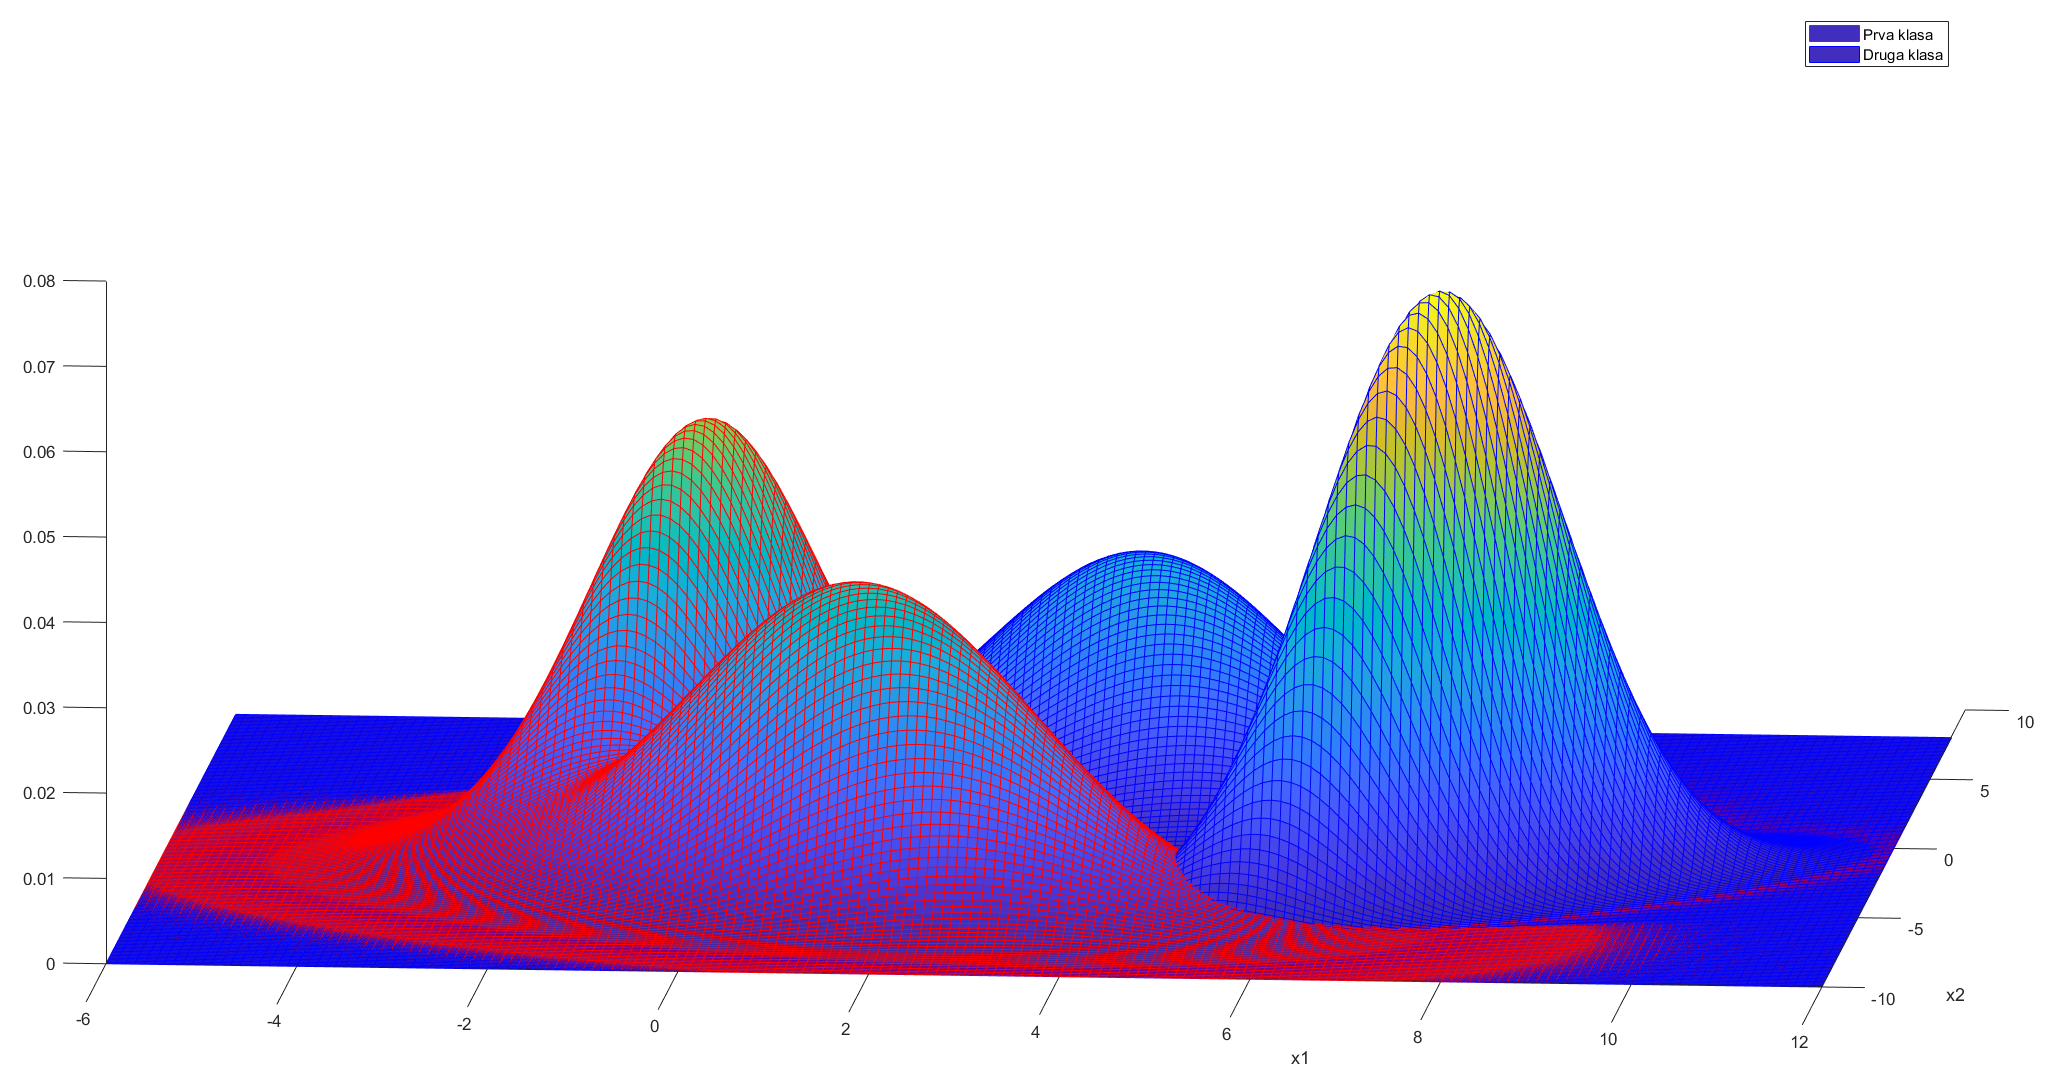
\includegraphics[scale=0.33]{pictures/2/FGV}
\caption{Функције густине вероватноће}\label{fig:FGV}
\end{figure}

\begin{figure}[htb!]
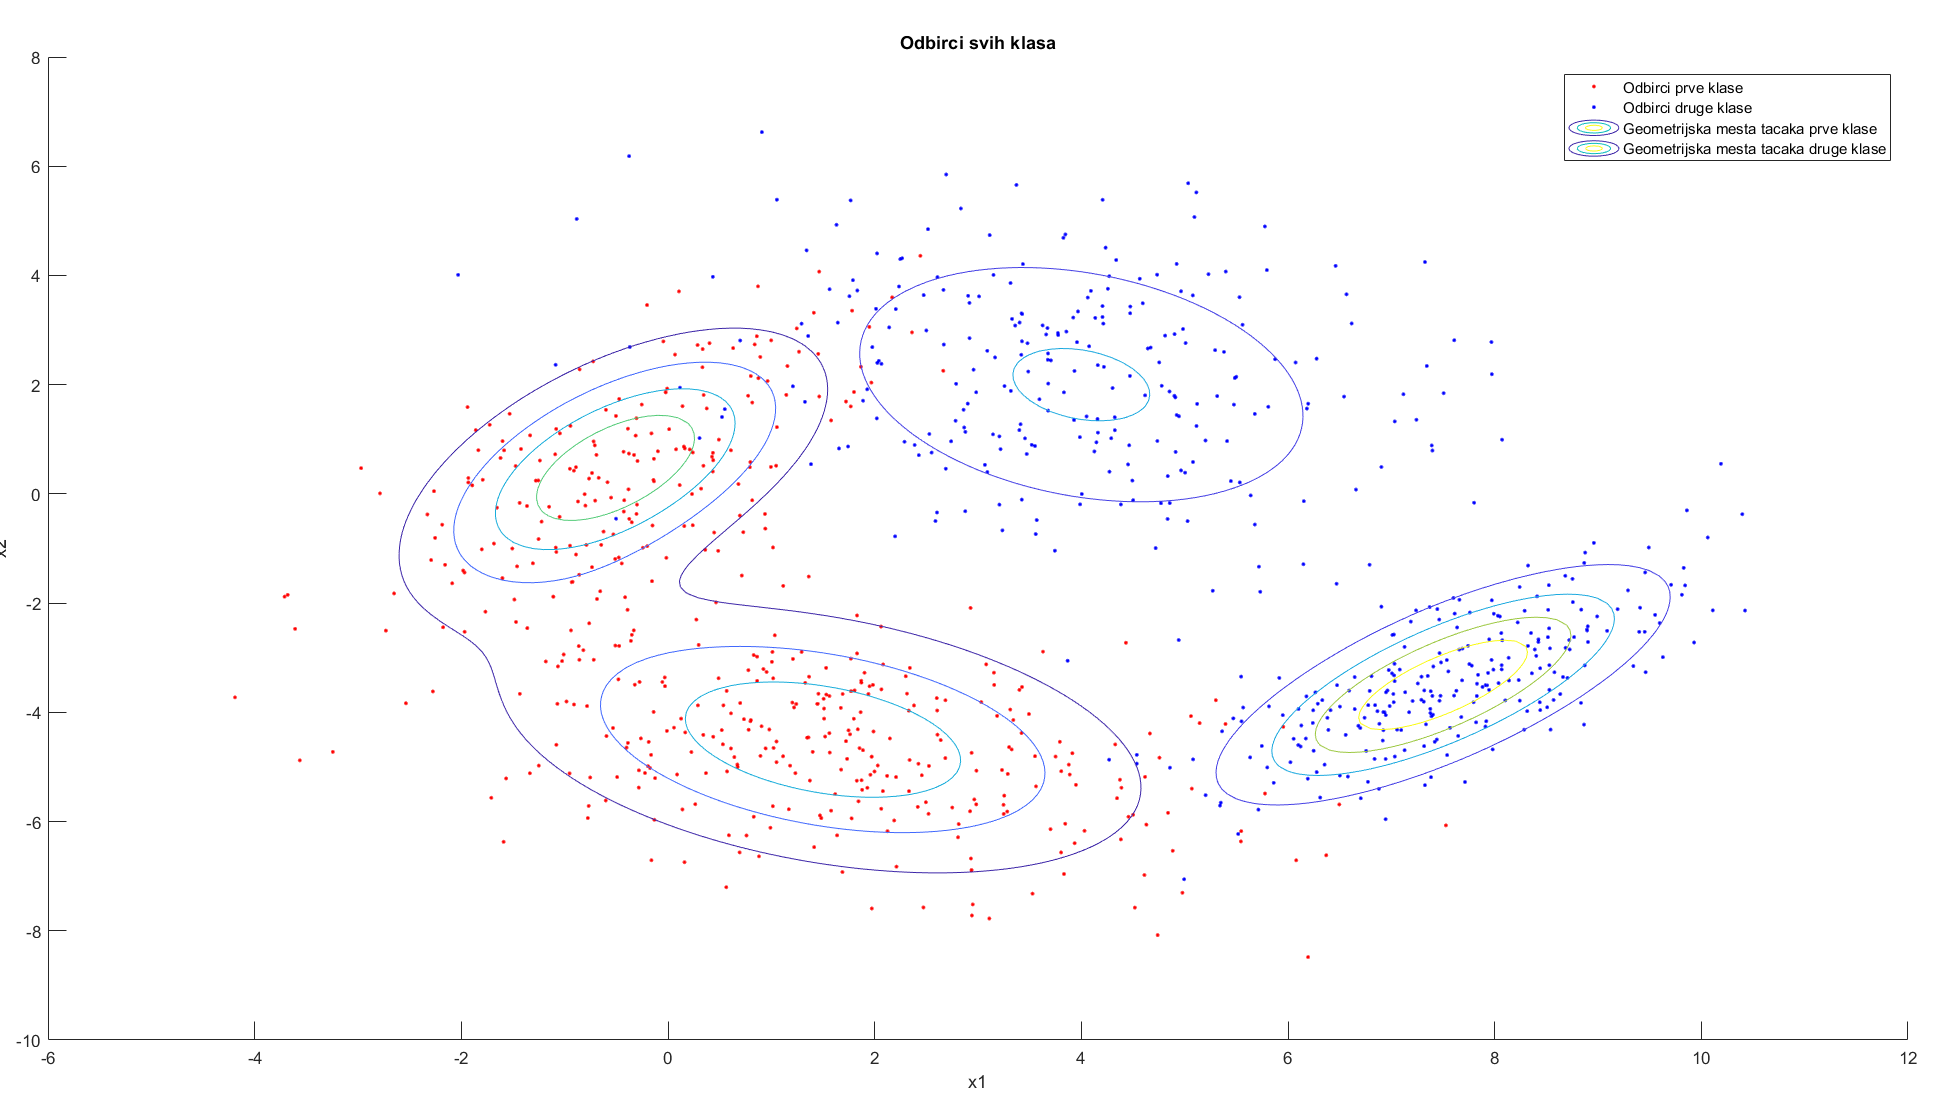
\includegraphics[scale=0.33]{pictures/2/FGVContour}
\caption{Функције густине вероватноће-геометријска места тачака}\label{fig:FGVContour}
\end{figure}
\newpage
\subsection{Бајесов класификатор минималне грешке}
Дати класификатор има следеће правило одлучивања:
$$h(X) = -ln(f_1(X) + ln(f_2(X)) < ln\left( \frac{P_1}{P_2}\right) \implies X \in \omega_1$$
$$h(X) = -ln(f_1(X) + ln(f_2(X)) >ln\left( \frac{P_1}{P_2}\right) \implies X \in \omega_2$$
где су $P_1, P_2$ априорне вероватноће појављивања класа. Како је број генерисаних тачака 500, важи $P_1 = P_2 = 0,5$, стога $h(X)= 0$. Геометријска места тачака, као и дискриминациона функција је дата на слици \ref{fig:Bayes}.

\begin{figure}[htb!]
\centering
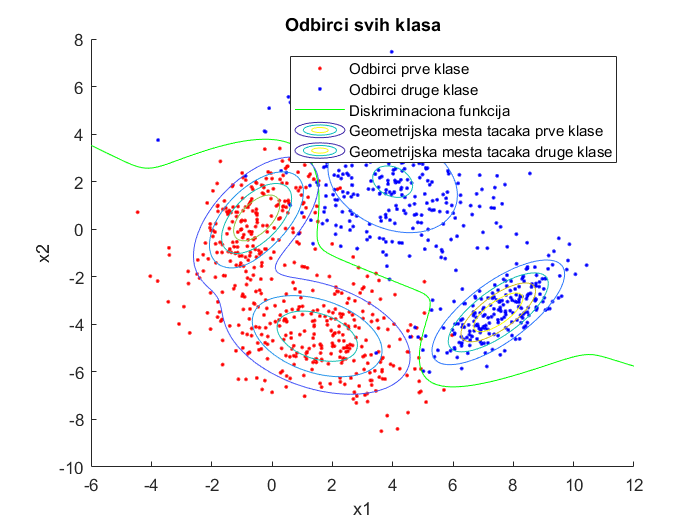
\includegraphics[scale=0.53]{pictures/2/Bayes}
\caption{Функције густине вероватноће, геометријска места тачака и дискриминациона линија}\label{fig:Bayes}
\end{figure}
На одсечку кода \ref{fun:genBayes} је приказано како је генерисана дискриминациона функција.
\begin{lstlisting}[caption={Генерисање дискриминационе функције},label={fun:genBayes}]
X1 = gausianMultimodalGenerate(P11, P12, M11, M12, S11, S12, num_points);
X2 = gausianMultimodalGenerate(P21, P22, M21, M22, S21, S22, num_points);

step = 0.1;
xIt = -6 : step : 12;
yIt = -10 : step : 8;

m = length(xIt);
n = length(yIt);

f1 = zeros(m, n);
f2 = zeros(m, n);
h = zeros(m, n);

[XItGrid, YItGrid] = meshgrid(xIt, yIt);

for i = 1 : m
    for j = 1 : n
        tempInput = [XItGrid(i, j) YItGrid(i, j)]';
        f1(i, j) = gausianMultimodal(tempInput, P11, P12, M11, M12, S11, S12);
        f2(i, j) = gausianMultimodal(tempInput, P21, P22, M21, M22, S21, S22);
        h(i, j) = log(f2(i, j)) - log(f1(i, j));
        
    end
end

f1Max = max(max(f1));
f2Max = max(max(f2));

figure(1);
hold on;    
plot(X1(:, 1), X1(:, 2), 'r.'); 
plot(X2(:, 1), X2(:, 2), 'b.');

xlabel('x1');
ylabel('x2');

title('Odbirci svih klasa');

contour(XItGrid, YItGrid, h, [0 0], 'g');
contour(XItGrid, YItGrid, f1, [0.8 * f1Max f1Max * 0.6 f1Max * 0.4 f1Max * 0.2]);
contour(XItGrid, YItGrid, f2, [0.8 * f2Max f2Max * 0.6 f2Max * 0.4 f2Max * 0.2]);

legend('Odbirci prve klase', 'Odbirci druge klase', 'Diskriminaciona funkcija',...
        'Geometrijska mesta tacaka prve klase', 'Geometrijska mesta tacaka druge klase');

\end{lstlisting}
Вероватноћа грешке првог и другог типа се рачунају по формули:
$$\varepsilon_1 = \int_{L_2} f_1(X)dX, \varepsilon_2 = \int_{L_1}f_2(X)dX,$$
При чему су $L1, L2$ области на које дели дискриминациона функција, при чему је $L1$ она област за коју густина вероватноће припадност класи 1 има већу вредност, за $L2$ обратно.
Пошто интеграл није решив, рачунао се методом правоугаоника (квадара). Функција из одсечка кода \ref{fun:epsilonEst} је имплементација методе правоугаоника(квадара).Вредност грешке првог типа је $3,7\%$ а другог типа је $3,8\%$.

\begin{lstlisting}[caption={Процена грешке},label={fun:epsilonEst}]
function [epsilon1,epsilon2] = errorEstimation(f1, f2, disFunction, num_rows, num_cols, step)
epsilon1 = 0;
epsilon2 = 0;

for i = 1 : num_rows
    for j = 1 : num_cols
        if (disFunction(i, j) < 0)
            epsilon2 = epsilon2+ f2(i, j) * step^2;
        else 
            epsilon1 = epsilon1 + f1(i, j) * step^2;
        end
    end
end

end
\end{lstlisting}

\subsection{Бајесово правило одлучивања минималне цене}
Класификацију ћемог поново извршити, али овога пута помоћу Бајесоовг правила одлучивања минималне цене. Тест је сличан Бајесовом, с тим да одговарајућих коефицијенти кажњавају грешке једног или другог типа, односно "дозвољавају" их. $c_{ij}$ цена одлуке $X \in \omega_i$ кад је заправо $X \in \omega_j$. Условна цена одлуке износи 
$$r_i(X) = c_{i1}q_1(X) + c_{i2}q_2(X),$$ тј.
$$r_1(X) < r_2(X) \implies X \in \omega_1$$
$$r_1(X) > r_2(X) \implies X \in \omega_2$$
Тада априорни ризик добија облик: $r(X) = min(r_1(X), r_2(X))$. Минимизацијом израза добија се:
$$\frac{f_1(X)}{f_2(X)} > \frac{(c_{12}-c_{22})P_2}{(c_{21} - c_{11})P_1} \implies X\in \omega_1$$
$$\frac{f_1(X)}{f_2(X)} < \frac{(c_{12}-c_{22})P_2}{(c_{21} - c_{11})P_1} \implies X\in \omega_2$$
Како је $P_2 = P_1$, и $h(X) = -ln(\frac{f_1(X)}{f_2(X)}$ добија се:
$$h(X) = ln(f_2(X) (c_{12} - c_{22})) - ln(f_1(X)(c_{21} - c_{11})) < 0 \implies X \in \omega_1$$
$$h(X) = ln(f_2(X) (c_{12} - c_{22})) - ln(f_1(X)(c_{21} - c_{11})) >0 \implies X \in \omega_2$$

Ако ставимо  $c_{11} = c_{22} = 0$ постављањем $c_{12}, c_{21}$ на одговарајуће вредности добијамо да се кажњава више одговарајући тип грешке (в. сл. \ref{fig:BayesMinimal}). У случају $c_{12} = 3, c_{21} = 1$ добијамо да је дискриминациона функција примакнута првој класи, што има смисла, јер се кажњава промашај ако је се претпоставило да је прва класа, а треба да је друга. Обратно, важи само за другу класу кад је $c_{21} = 3, c_{12} =1$. Кад је $c_{21}=c_{12}$ тест постаје Бајесов класификатор минималне грешке (што се и види на слици).
Грешке су рачунају истом функцијом као и Бајесов класификатор, при чему у првом случају је грешка прве врсте $0, 072$, а друге $0, 018$, а у другом $0, 017$ односно $0,072$. Претходно је такође логично јер је у првом случају дискриминациона функција близу прве класе и више ће бити погрешно класификованих њених одбирака у другу класу. 


\begin{figure}[htb!]
\centering
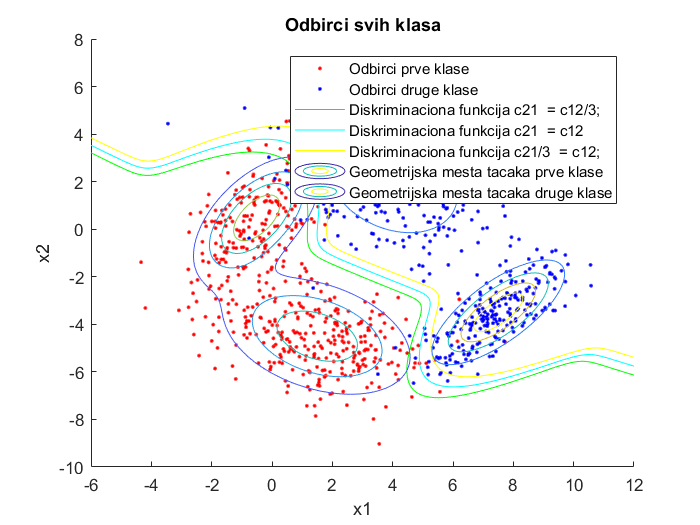
\includegraphics[scale=1]{pictures/2/BayesMinimal}
\caption{Тест минималне цене}\label{fig:BayesMinimal}
\end{figure}
\subsection{Волдов секвенцијални тест}

У претходно обрађеним класификаторима одлука је доношена само на основу информација које тренутно се поседују. Али у многим практичним применама информације стижу секвенцијално и њихов број се увећава. Фамилија секвенцијалних класификатора у озбир узима и претходна мерења. Један од њих је Волдов тест. Он доноси одлуку након коначног броја мерења када вероватноћа грешке спадне на жељене нивое $\varepsilon_1$ и $\varepsilon_2$.

Дефинишемо $s$ који представља негативни логаритам здружене функције густине вероватноће свих мерења и узимамо претпоставку да су оне независне:

$$s_m = -ln\frac{f_1(X_1, ..., X_m)}{f_2(X_1, ..., X_m)} = \sum_{i=1}^m \left( -ln\frac{f_1(X_i)}{f_2(X_i)}\right) = \sum_{i=1}^mh(X_i)$$

Волдов тест функционише:
\begin{enumerate}[1)]
\item $s_m \leq a \implies X \in \omega_1$
\item $a < s_m < b \implies $ узети следеће мерење
\item $s_m \geq b \implies X \in \omega_2$
\end{enumerate}

Границе $a$ и $b$ су директно повезане са $\varepsilon_1$ и $\varepsilon_2$ и износе:
$a=-ln\frac{1-\varepsilon_1}{\varepsilon_2}$, $b =-ln\frac{\varepsilon_1}{1-\varepsilon_2}$

Код који имплементира је одсечак кода \ref{fun:waldoTest}. Можемо да видимо да код понавља $testCases$ пута Валдов тест да би усредњио број итерација неопходан за детекцију класе којој припада јер се насумично узимају тачке из одређене класе $X$. 

\begin{lstlisting}[caption={Одређивање припадностие},label={fun:waldoTest}]
function [classIdx, i] = waldosTest(X, epsilon1, epsilon2, P11, P12, P21, P22, ...
                                        M11, M12, M21, M22, S11, S12, S21, S22)
a = -log((1 - epsilon1) / epsilon2);
b = -log(epsilon1 / ( 1 - epsilon2));

num_points = size(X, 1);
testCases = 25;
sumI = 0;

for testIdx = 1 : testCases
    idx = randperm(num_points);

    i = 1;

    s = -log(gausianMultimodal(X(idx(i), :)', P11, P12, M11, M12, S11, S12)) + ...
           log(gausianMultimodal(X(idx(i), :)', P21, P22, M21, M22, S21, S22)) ;
    
    while ((i + 1 <= num_points) && (s < b) && (s > a))
        i = i + 1;
        s = s + -log(gausianMultimodal(X(idx(i), :)', P11, P12, M11, M12, S11, S12)) + ...
           log(gausianMultimodal(X(idx(i), :)', P21, P22, M21, M22, S21, S22));
    end

    sumI = sumI + i;

    if (s <= a)
        classIdx = 1;
    elseif (s >= b)
        classIdx = 2;
    else 
        classIdx = 0;
    end

end
i = sumI / testCases;

end
\end{lstlisting}


Зависност броја потребних одбирака из прве, односно друге класе је:
$$E\{m|\omega_1\} = \frac{a(1-\varepsilon_1) + b\varepsilon_1}{\eta_1}=\frac{ln\frac{\varepsilon_2}{1-\varepsilon_1}(1-\varepsilon_1) + ln\frac{1-\varepsilon_2}{\varepsilon_1} \varepsilon_1}{\eta_1}$$
$$E\{m|\omega_2\} = \frac{b(1-\varepsilon_2) + a\varepsilon_2}{\eta_2}=\frac{ln\frac{1-\varepsilon_2}{\varepsilon_1}(1-\varepsilon_2) + ln\frac{\varepsilon_2}{1-\varepsilon_1} \varepsilon_2}{\eta_2},$$
при чему је $\eta_i =E\{h(X)|\omega_i\} = \int_{-\infty}^{+\infty}hf_h(h|\omega_i)dh $. Проценићемо израз само један израз $E\{m|w_i\}$ јер је други аналоган. Прво морамо да проценимо $\eta_1$, то је обављено коришћењем исечка кода \ref{fun:estH}, који се своди на метод хистограма тако што множимо одговарајућу функцију густине вероватноће са одговарајућом вредношћу. Добија се да је за $\omega_1$ вредност $\eta_1 =-7,263$. Хистограм је дат на слици \ref{fig:WaldoHisto}. Добијена зависност усредњеног броја одбирака од усвојене вероватноће грешке је на сликама \ref{pic:eps1Dep} и \ref{pic:eps2Dep}.

\begin{figure}[htb!]
\centering
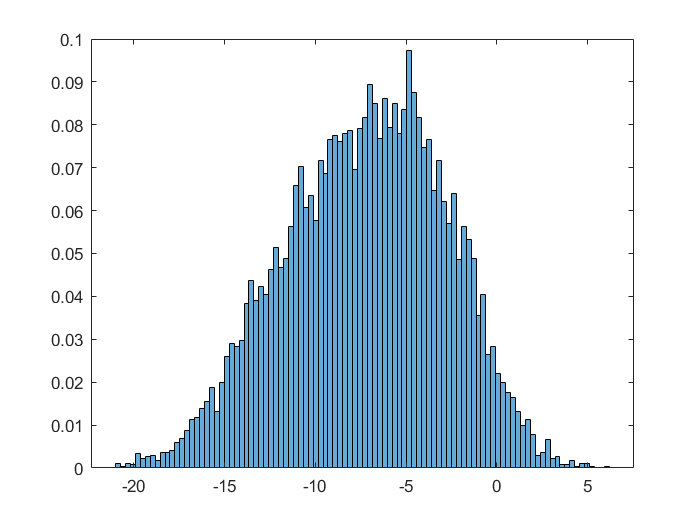
\includegraphics[scale=1]{pictures/2/histogram}
\caption{Хистограм процењене густине вероватноће}\label{fig:WaldoHisto}
\end{figure}


\begin{lstlisting}[caption={Процена условног h},label={fun:estH}]
function [expValCond, hApprox] = condProbDiscApprox(P11, P12, P21, P22, M11, M12, M21, M22, S11,...
                                                    S12, S21, S22)
num_points = 10000;
X1Approx = gausianMultimodalGenerate(P11, P12, M11, M12, S11, S12, num_points);
m = size(X1Approx, 1);
hApprox = zeros(m, 1);

for i = 1 : m
    tempInput = X1Approx(i, :)';
    f1Approx = gausianMultimodal(tempInput, P11, P12, M11, M12, S11, S12);
    f2Approx = gausianMultimodal(tempInput, P21, P22, M21, M22, S21, S22);
    hApprox(i) = log(f2Approx) - log(f1Approx);
end

[condProb, bins] = histcounts(hApprox, 100, 'Normalization', 'pdf');

expValCond = 0;
step = bins(2) - bins(1);
for i = 1 :  length(condProb)
    x = (bins(i) + bins(i + 1)) /2;
    expValCond = expValCond + x * condProb(i) * step;
end

end

\end{lstlisting}

\begin{figure}[htb!]\caption{Графици зависности}
\begin{subfigure}{.6\textwidth}
\centering
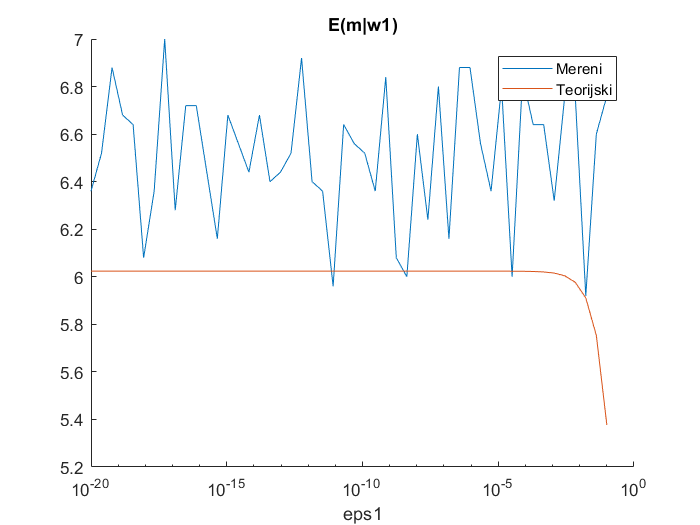
\includegraphics[width=1\linewidth]{pictures/2/WaldoE1}
\caption{$\varepsilon_2 = 10^-20$, зависност у односу на $\varepsilon_1$}\label{pic:eps1Dep}
\end{subfigure}
\begin{subfigure}{.55\textwidth}
\centering
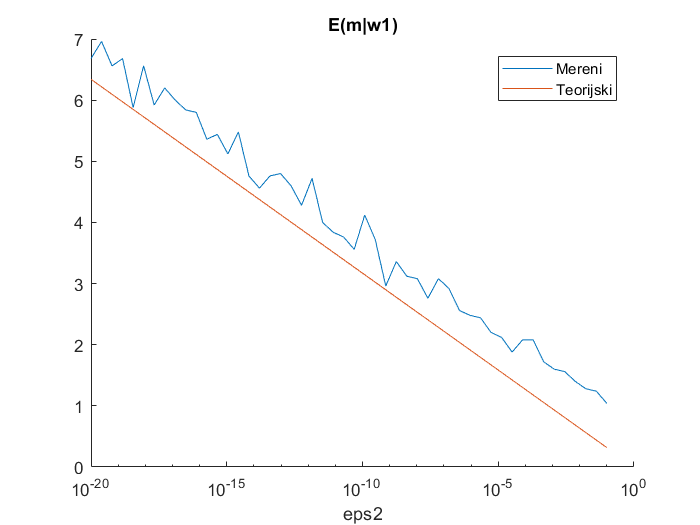
\includegraphics[width=1\linewidth]{pictures/2/WaldoE2}
\caption{$\varepsilon_1 = 10^-20$, зависност у односу на $\varepsilon_2$}\label{pic:eps2Dep}
\end{subfigure}
\end{figure}

Са последње две слике се  уочава да очекивани број одбирака из прве класе за доношење одлуке  зависи од вероватноће грешке другог типа, док вероватноћа грешке првог типа скоро па нема утицај. Аналогно за другу класу, потребан број одбирака из друге класе  зависи од $\varepsilon_1$, док скоро уопште не зависи од $\varepsilon_2$
\newpage
\section{Трећи домаћи задатак}
\renewcommand{\lstlistingname}{Одсечак кода}%
\begin{enumerate}[1.]
\item Генерисати две класе дводимензионалних облика. Изабрати функцију густине вероватноће облика тако да класе буду линеарно сепарабилне.
\begin{enumerate}[a)]
\item За тако генерисане облике извршити пројектовање линеарног класификатора једном од три итеративне процедуре.
\item Поновити претходни поступак методом жељеног излаза. Анализирати утицај елемената у матрици жељених излаза на коначну форму линеарног класификатора.
\end{enumerate}
\item Генерисати две класе дводимензионалних облика које су сепарабилне, али не линеарно, па испројектовати квадратни класификатор методом по жељи.
\end{enumerate}
\subsection{Линеарни класификатор}
\subsubsection{Генерисање класа}
За почетак генерисаћемо одбирке двеју дводимензионалних класа чије су функције густине вероватноће у облику бимодалних Гаусових расподела:


$$f_1(X) = P_{11} N(M_{11}, \Sigma_{11}) + P_{12} N(M_{12}, \Sigma_{12})$$
$$f_2(X) = P_{21} N(M_{21}, \Sigma_{21}) + P_{22} N(M_{22}, \Sigma_{22}),$$
при чему вероватноће, средње вредности и коваријационе матрице имају следеће вредности:
$$P_{11} = 0,6,  M_{11} = \begin{bmatrix}
   0,5\\
   -7
\end{bmatrix}, 
S_{11} = \begin{bmatrix}
				   3,5 & -1\\
				   -1 & 2,2
				\end{bmatrix},
P_{12} = 0,4,  M_{12} = \begin{bmatrix}
										   -1\\
										   -1
										\end{bmatrix}, 
S_{12} = \begin{bmatrix}
				   1,3 & -0,9\\
			   	-0,9 &  2
				\end{bmatrix}
$$				
$$P_{21} = 0,45,  M_{21} = \begin{bmatrix}
   7,5\\
   -3,5
\end{bmatrix}, 
S_{21} = \begin{bmatrix}
				   4 & 1,1\\
				   1,1 & 4
				\end{bmatrix},
P_{22} = 0,55,  M_{22} = \begin{bmatrix}
										   4\\
										   2
										\end{bmatrix}, 
S_{22} = \begin{bmatrix}
				   3 & -0,8\\
			   	-0,8 &  3
				\end{bmatrix}
$$

Добијене класе су на слици \ref{fig:linClass}.
\begin{figure}[htb!]
\centering
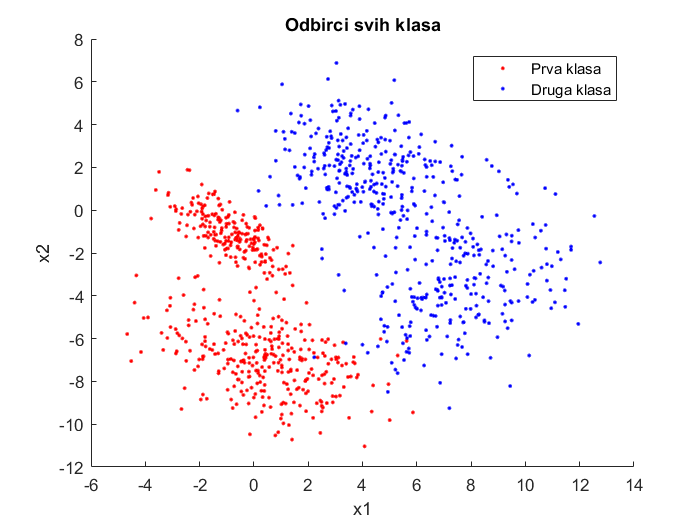
\includegraphics[scale=.5]{pictures/3/LinClass}
\caption{Одбирци}\label{fig:linClass}
\end{figure}
\subsubsection{Пројектовање линеарног класификатора методом ресупституције}
Линеарни класификатор је један од најједноставнијих класификатора, Иако у већини случајева није оптималан јер класе не морају да буду линеарно сепарабилне, често се користи због једноставности. Дискриминациона функција је линеарна и правило одлучивања гласи:
$$h(X) = V^T + v_0 < 0 \implies X \in \omega_1$$
$$h(X) = V^T + v_0 >0 \implies X \in \omega_2$$
Метод који је коришћен је метод ресупституције. Првобитно су процењени вектори средњих вредности $M1Approx, M2Approx$ и коваријационе матрице $S1Approx, S2Approx$, то је коришћено одсечком кода \ref{piece:expVarApprox}.

\begin{lstlisting}[caption={Процена математичког очекивања и ковариационе матрице},label={piece:expVarApprox}]
M1Approx = mean(X1)';
M2Approx = mean(X2)';

S1Approx = cov(X1);
S2Approx = cov(X2); 
\end{lstlisting}
Потом се у сваком кораку мења вредност параметра $s \in \left[ 0, 1\right] $,
и за свако $s$ одреди се вектор :
$$V=\left[ s * S1Approx + (1 - s)*S2Approx\right]^{-1}(M2Approx - M1Approx)$$
Потом се вектор $X$ пројектује на вектор $V$:
$$y_j^{(i)} = V^T X_j^{(i)}, i = 1, 2, j=1, ... N_i$$
где је $N_i$ број облика из $i$-те класе, а $X_j^{(i)}$ $j-$ти обучавајући вектор из $i$-те класе. Затим се $v_0$ мења да се добије најмања грешка. Мења се у опсегу $\left[ -max(max(y_j^{(i)}, max(y_j^{(2)})), -min(min(y_j^{(1)}, min(y_j^{(2)}))\right]$. На крају процедуре бира се оно $s$ за које је број погрешно класификованих објеката (односно грешка) најмањи. 
На слици \ref{fig:sDep} имамо како се $s$ мења у интервалу $\left[0, 1\right]$. Можемо да приметимо да је минимална вредност било која између $0$ и $0, 15$, стога бирамо $0$. 

\begin{figure}[htb!]
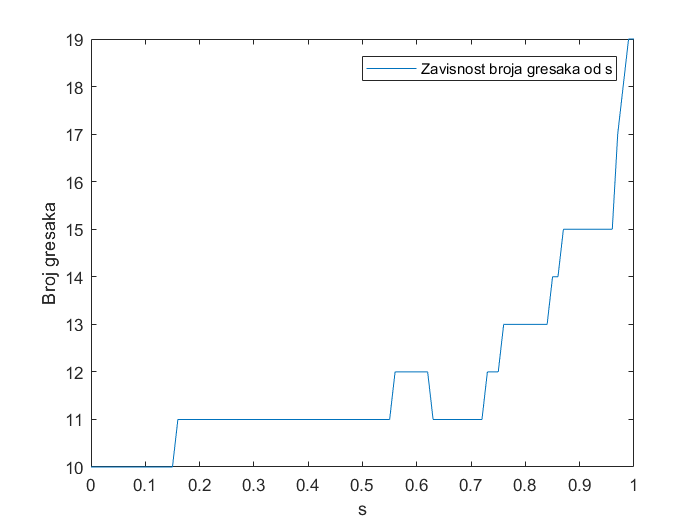
\includegraphics[scale=.6]{pictures/3/sDep}
\centering
\caption{Зависност броја грешака од $s$}\label{fig:sDep}
\end{figure}
За овај случај се добија $V =[1,5254 1.1170]^T, v_0 = -0,6212$ што се види на слици \ref{fig:linClassDisc}. Такође треба приметити да је број грешака 10 што значи да је грешка $1\%$.

\begin{figure}[htb!]
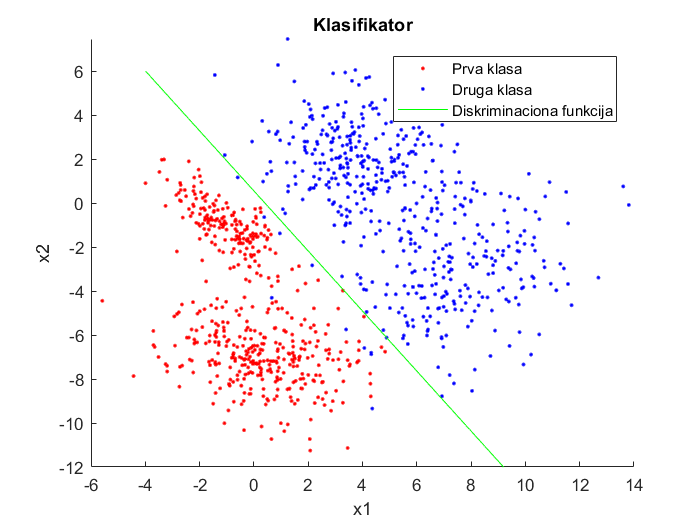
\includegraphics[scale=.6]{pictures/3/LinClassDisc}
\centering
\caption{Одбирци}\label{fig:linClassDisc}
\end{figure}

Код којим је одрађено претходно је одсечак кода \ref{piece:linClassProj}.

\begin{lstlisting}[caption={Пројектовање линеарног класификатора},label={piece:linClassProj}]
step = 0.01;
s = 0 : step : 1;
num_s = length(s);
for i = 1 : num_s
    V = (s(i) * S1Approx  + (1 - s(i)) * S2Approx) \ (M2Approx - M1Approx);
    Y1 = X1 * V;
    Y2 = X2 * V;
    
    downLimit = -max(max(Y1), max(Y2));
    upLimit = -min(min(Y1), min(Y2));
    
    V0 = downLimit : step : upLimit;
    
    minError = size(Y1, 1) + size(Y2, 1);
    minIdx = 0;
    
    V0Num = length(V0);
    
    for j = 1 : V0Num
        v0 = V0(j);
        wrongClass1 = nnz(Y1 > -v0);
        wrongClass2 = nnz(Y2 < -v0);
        wrongClass = wrongClass1 + wrongClass2;
        if (wrongClass < minError)
            minError = wrongClass;
            minIdx = j;
        end
    end
    epsilon(i) = minError;
    V0Min(i) = V0(minIdx);
    
end

[epsilon, idx] = min(epsilon);

sVal = s(idx);

V = (sVal * S1Approx  + (1 - sVal) * S2Approx) \ (M2Approx - M1Approx)
v0 = V0Min(idx)

\end{lstlisting}

\subsubsection{Метод жељеног излаза}
Поновићемо поступак пројектовања линеарног класификатора над датим класама, али овога пута методом жељеног излаза. Код ове методе линија класификациона линија се формаиа тако да за исправно класификован објекат увек буде позитивна:
$$h(X) = -V^T - v_0 > 0 \implies X \in \omega_1$$
$$h(X) = V^T + v_0 > 0 \implies X \in \omega_2$$
Да би се то постигло уводи се нови улазни вектор:
$$Z=[-1 -X_1 .... -X_n]^T,X\in \omega_1$$
$$Z=[1 X_1 .... X_n]^T,X\in \omega_2$$
Проблем се своди на одређивање вектора $W_{(n+1)\times1}$ за који ће што више одбирака $Z$ да испуне релацију $h(Z) = W^TZ > 0$. Критеријумска функција која је најзахвалнија за минимизацију је:
$$\overline{\varepsilon^2} = \frac{1}{N} \sum_{j=1}^N (W^TZ_j - \gamma(Z_j))^2$$
Применом парцијалног извода на њу, и изједначавањем са 0, добија се $U^TW = \Gamma$.
Дата једначина се решава псеудоинверзијом:
$$W = (UU^T)^{-1}U \Gamma,$$
где је $U=[Z_1 Z_2 ... Z_n]$ матрица узорака, а $\Gamma=[\gamma(Z_1) ... \gamma(Z_n)]]^T$ матрица жељених излаза.
Често се за матрицу жељених излаза узима јединични вектор. Одсечак кода \ref{piece:linClassExp} имплементира методу жељеног излаза. 

\begin{lstlisting}[caption={Метода очекиваног излаза},label={piece:linClassExp}]
U = zeros(3, num_points * 2);
G = ones(num_points * 2, 1);
for i = 1 : num_points
    U(:, 2 * i - 1) = [-1 -X1(i, :)];
    U(:, 2 * i) = [1 X2(i, :)];
end

W = U * U' \ U * G;

xIt = -6 : 0.01 : 14;
yIt = -12 : 0.01 : 6;
hExpectedOutput = zeros(length(xIt), length(yIt));
for i = 1 : length(xIt)
    for j = 1 : length(yIt)
        hExpectedOutput(i, j) = [1 xIt(i) yIt(j)] * W;
    end
end
\end{lstlisting}

Добијена функција је $h(X) = -0,2581 + 0,20417_1 + 0,1166x_2$ је приказан на слици \ref{fig:expClassNorm}.
Грешка се рачуна функцијом чији је одсечак кода \ref{piece:linClassExpErr}. 
\begin{figure}[htb!]
\centering
\includegraphics[scale=1]{pictures/3/ExpClassNorm}
\caption{Дискриминациона функција код методе очекиваног излаза}\label{fig:expClassNorm}
\end{figure}

\begin{lstlisting}[caption={Метода очекиваног излаза - грешка},label={piece:linClassExpErr}]
function [epsilon1, epsilon2, epsilon] = errorEstimationEO(U, W, num_points)
    Y = U' * W;
    epsilon = numel(Y(Y < 0)) / (2 * num_points);
    epsilon1 = 0;
    epsilon2 = 0;
    for i = 1 : num_points
        epsilon1 =  (Y(2 * i - 1) < 0) + epsilon1;
        epsilon2 = (Y(2 * i) < 0) + epsilon2;
    end
    epsilon1 = epsilon1 / num_points;
    epsilon2 = epsilon2 / num_points;
end
\end{lstlisting}
Добијене грешке су $\varepsilon_2 = 0,034, \varepsilon_1=0,004, \varepsilon = 0.019$.
Можемо да приметимо да је $\varepsilon_2$ много већа него $\varepsilon_1$. Ако бисмо желели да је смањимо науштрб грешке $\varepsilon_1$ онда бисмо очекиване излазе за елементе који припадају другој класи морали да повећамо. Када то урадимо добија се$\varepsilon_1 = 0.008, \varepsilon=0,024, \varepsilon=0,016$. На слици \ref{fig:expClassNorm} се налази и новодобијена функција. Уопштено ако имамо неку грешку која је већа и желимо да је умањимо методом жељеног излаза, само треба да повећамо жељене излазе за тип грешке који желимо да смањимо.

Ако бисмо желели да минимизујемо свеукупну грешку тад би свим тачкама у близини дискриминационе функције требали да повећамо вредност.  Ако итеративно понављамо дату операцију повећавања добијемо низ дискриминационих функција које конвергирају као на слици \ref{fig:expClassConv} жутој линији. Грешка се смањује и $\varepsilon =0,015$ након ове операције, што је мање него првобитна свеукупна грешка. Одсечак кода \ref{piece:linClassConv} приказује имплементацију претходно наведеног. 
\begin{figure}[htb!]
\centering
\includegraphics[scale=1]{pictures/3/ExpClassConv}
\caption{Низ дискриминационих функција код методе очекиваног излаза}\label{fig:expClassConv}
\end{figure}

\begin{lstlisting}[caption={Метода очекиваног излаза - конвергирање},label={piece:linClassConv}]
U = zeros(3, num_points * 2);
G = ones(num_points * 2, 1);
for i = 1 : num_points
    U(:, 2 * i - 1) = [-1 -X1(i, :)];
    U(:, 2 * i) = [1 X2(i, :)];
end
for t = 1 : 10

    W = U * U' \ U * G;
    xIt = -6 : 0.01 : 14;
    yIt = -12 : 0.01 : 6;
    hExpectedOutput = zeros(length(xIt), length(yIt));
    for i = 1 : length(xIt)
        for j = 1 : length(yIt)
            hExpectedOutput(i, j) = [1 xIt(i) yIt(j)] * W;
        end
    end

    [e1, e2, e] = errorEstimationEO(U, W, num_points);

    fprintf("ExpClose : Greska %.3f Greska1 : %.3f Greska 2 %.3f\n", e, e1, e2);
    if (t == 10)
        contour(xIt,yIt,hExpectedOutput',[0 0],'y');
    else
        contour(xIt,yIt,hExpectedOutput',[0 0],'g');
    end
    Y = U' * W;
    idx = find(Y(1:num_points) < 0.1);
    for i = 1:length(idx)
        G(idx(i)) = 10;
    end
end
\end{lstlisting}

\subsection{Kвадратни класификатор}

Представља сложељнију форму класификатора. Користи се кад две класе нису линеарно сепарабилне. Општа форма квадратног класификатора је:
$$h(X) = X^TQX + V^TX + v_0 < 0 \implies X\in \omega_1$$
$$h(X) = X^TQX + V^TX + v_0 > 0 \implies X\in \omega_2$$
Да би се могао пројектовати неком од постојећих метода, треба да се изврши првидна линеаризација квадратног класификатора. То ћемо учинит на следећи начин:
$$h(X) = q_{11} x_1^2 + q_{22}x_2^2 + q_{12}x_1x_2  + v_1x + v_2x_2 + v_0 = W^TZ > 0 $$
где је улазни вектор 
$$Z=[-1 -x_1 -x_2 -x_1x_2 -x_1^2 -x_2^2]^T, X\in \omega_1$$
$$Z=[1 \, x_1 \, x_2\,  x_1x_2\,  x_1^2\,  x_2^2]^T, X\in \omega_2$$
вектор параметара $W = [v_0 v_1 v_2 q_{12} q_{11} q_{22}$

За почетак генерисаћемо одбирке двеју дводимензионалних класа чије су функције густине вероватноће у облику бимодалних Гаусових расподела:
\\
$$f_1(X) = P_{11} N(M_{11}, \Sigma_{11}) + P_{12} N(M_{12}, \Sigma_{12})$$
$$f_2(X) = P_{21} N(M_{21}, \Sigma_{21}) + P_{22} N(M_{22}, \Sigma_{22}),$$
при чему вероватноће, средње вредности и коваријационе матрице имају следеће вредности:
$$P_{11} = 0,6,  M_{11} = \begin{bmatrix}
   0,5\\
   -7
\end{bmatrix}, 
S_{11} = \begin{bmatrix}
				   3,5 & -1\\
				   -1 & 2,2
				\end{bmatrix},
P_{12} = 0,4,  M_{12} = \begin{bmatrix}
										   12\\
										   6
										\end{bmatrix}, 
S_{12} = \begin{bmatrix}
				   1,3 & -0,9\\
			   	-0,9 &  1.2
				\end{bmatrix}
$$				
$$P_{21} = 0,45,  M_{21} = \begin{bmatrix}
   7,5\\
   -3,5
\end{bmatrix}, 
S_{21} = \begin{bmatrix}
				   4 & 1,1\\
				   1,1 & 4
				\end{bmatrix},
P_{22} = 0,55,  M_{22} = \begin{bmatrix}
										   4\\
										   2
										\end{bmatrix}, 
S_{22} = \begin{bmatrix}
				   3 & -0,8\\
			   	-0,8 &  3
				\end{bmatrix}
$$
Применом методе псудоинверзије добијамо да ус вектор параметара и дискриминациона функција:
$$W = [0,7240,\,0,0622\,\,0,1785\,\, -0,0310\,\, -0,0061\,\, 0,0105]$$
$$h(X) = -0,7240 +0,0622x_1+0,1785x_2 -0,0310x_1x_2 -0,0061x_1^2 +0,0105x_2^2$$
Добијају се грешке $\varepsilon=0,013, \varepsilon_1 = 0,024, \varepsilon_2=0,002$. Дискриминациона функција и одбирци су приказани на слици \ref{fig:quadClass}.

\begin{figure}[htb!]
\centering
\includegraphics[scale=1]{pictures/3/QuadClass}
\caption{Квадратни класификатор}\label{fig:quadClass}
\end{figure}
\newpage
\newpage
\section{Четврти домаћи задатак}
\begin{enumerate}[1.]
\item Генерисати по $N=500$ дводимензионалних одбирака из четири класе које ће бити линеарно сепарабилне. Препоручује се да то буду гаусовски расподељени дводимензионални облици. Изабрати једну од метода за кластеризацију (C-mean метод, метод квадратне декомпозиције, метод максималне веродостојности или метод грана и граница) и применити је на формиране узорке класа. Извршити анализу осетљивости изабраног алгоритма на почетну кластеризацију, као и средњи број потребних итерација. Такође извршити анализе случаја када се априорно не познаје број класа.
\item Генерисати по $N=500$ дводимензионалних одбирака из две класе које су нелинеарно сепарабилне. Изабрати једну од метода за кластеризацију које су применљиве за нелинеарно сепарабилне класе (метод квадратне декомпозиције или метод максималне веродостојности) и поновити анализу из претходне тачке.
\end{enumerate}
\subsection{C-Mean алгоритам}
\subsubsection{Генерисање одбирака}
За почетак генерисаћемо одбирке четири дводимензионалних класа чије су функције густине вероватноће у облику  гаусовских расподела:


$$f_1(X) = N(M_{1}, \Sigma_{1}), f_2(X) = N(M_{2}, \Sigma_{2}), f_3(X) = N(M_{3}, \Sigma_{3}),f_4(X) = N(M_{4}, \Sigma_{4})$$
при чему вероватноће, средње вредности и коваријационе матрице имају следеће вредности:
$$ M_{1} = \begin{bmatrix}
   -4\\
   -4
\end{bmatrix}, 
 M_{2} = \begin{bmatrix}
   4\\
   4
\end{bmatrix}, 
 M_{3} = \begin{bmatrix}
   4\\
   -4
\end{bmatrix}, 
 M_{1} = \begin{bmatrix}
   -4\\
   4
\end{bmatrix}, 
 M_{4} = \begin{bmatrix}
   -4\\
   4
\end{bmatrix}, 
$$				
$$S_{1} = \begin{bmatrix}
				   1,5 & 1\\
				   1 & 2,5
				\end{bmatrix},
S_{2} = \begin{bmatrix}
	2 & 1\\
	1 & 2
\end{bmatrix},
S_{1} = \begin{bmatrix}
	1,5 & -1\\
	-1 & 1,5
\end{bmatrix},
S_{1} = \begin{bmatrix}
	2 & -1\\
	-1 & 2
\end{bmatrix}$$

\renewcommand{\lstlistingname}{Одсечак кода}%
Добијају се 4 класе одбирака као на слици \ref{fig:Odbirci}
\begin{figure}[htb!]
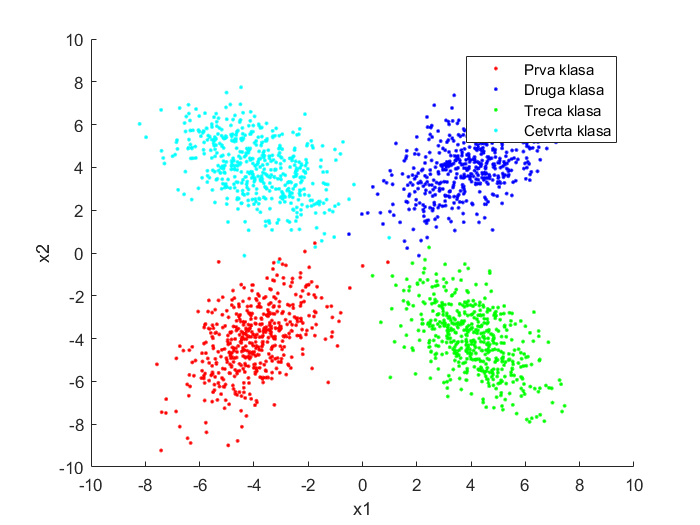
\includegraphics[scale=.8]{pictures/4/Odbirci}
\caption{Одбирци}\label{fig:Odbirci}
\end{figure}

\subsubsection{Алгоритам}
Кластеризацију над датим скупомо података ћемо извршити уз помоћ C-mean алгоритма. Једна од предности ове методе су њена једноставност, могућност стохастичке почетне кластеризације. Међутим, има и одређених ограничења. Кластери су поељени део по део линеарним линијама, што ограничава примену ове методе на линеарно сепарабилне класе. Такође, захтева априорно знање о броју кластера и не гарантује глобалну конвергенцију.

Одсечак кода \ref{fun:cMean} имплементира c-Mean алгоритам.


\begin{lstlisting}[caption={C-Mean функција},label={fun:cMean}]
function [num_it, critFun] = cMean(X1, X2, X3, X4, num_points, num_classes, apPer, drawFigure)

chunkRand = floor((1 - apPer) * num_points);
chunkApp = num_points - chunkRand;

Z = [X1(1 : chunkRand, :); X2(1 : chunkRand, :); ...
     X3(1 : chunkRand, :); X4(1 : chunkRand, :);];

num_points_all = 4 * chunkRand;

idx = randperm(num_points_all);
chunk_size = floor(num_points_all / num_classes);

Y1 = Z(idx(1 : chunk_size), :);
Y1App = X1(chunkRand + 1 : num_points, :);
Y1 = [Y1App; Y1];
Y2 = Z(idx(chunk_size + 1:2 * chunk_size), :);
Y2App = X2(chunkRand + 1 : num_points, :);
Y2 = [Y2App; Y2];
Y3 = [];
Y3App = [];
Y4 =[];
Y4App = [];
Y5 =[];
Y5App = [];
if (num_classes > 2)
    Y3 = Z(idx(2 * chunk_size + 1:3 * chunk_size), :);
    Y3App = X3(chunkRand + 1 : num_points, :);
    Y3 = [Y3App; Y3];
end 
if (num_classes > 3)
    Y4 = Z(idx(3 * chunk_size + 1:4 * chunk_size), :);
    Y4App = X4(chunkRand + 1 : num_points, :);
    Y4 = [Y4App; Y4];
end
if (num_classes > 4)
    Y5 = Z(idx(4 * chunk_size + 1:5 * chunk_size), :);
end
run = 1;

it = 0;

while (run && it < 50)
    it = it + 1;
    M1 = mean(Y1);
    M2 = mean(Y2);
    M3 = mean(Y3);
    M4 = mean(Y4);
    M5 = mean(Y5);
    
    if (size(M1, 2) == 1)
        M1 = [realmax realmax];
    end 
    if (size(M2, 2) == 1)
        M2 = [realmax realmax];
    end 
    if (size(M3, 2) == 1)
        M3 = [realmax realmax];
    end 
    if (size(M4, 2) == 1)
        M4 = [realmax realmax];
    end 
    if (size(M5, 2) == 1)
        M5 = [realmax realmax];
    end 
    clear X1 X2 X3 X4;
    
    M = [M1; M2; M3; M4; M5];
    
    [X11, X21, X31, X41, X51, changed1] = reCluster(Y1(chunkApp + 1: end, :), M, 1);
    [X12, X22, X32, X42, X52, changed2] = reCluster(Y2(chunkApp + 1: end, :), M, 2);
    [X13, X23, X33, X43, X53, changed3] = reCluster(Y3(chunkApp + 1: end, :), M, 3);
    [X14, X24, X34, X44, X54, changed4] = reCluster(Y4(chunkApp + 1: end, :), M, 4);
    [X15, X25, X35, X45, X55, changed5] = reCluster(Y5(chunkApp + 1: end, :), M, 5);
    run = changed1 | changed2 | changed3 | changed4 | changed5;
    Y1 = [Y1App; X11; X12; X13; X14; X15];
    Y2 = [Y2App; X21; X22; X23; X24; X25];
    Y3 = [Y3App; X31; X32; X33; X34; X35];
    Y4 = [Y4App; X41; X42; X43; X44; X45];
    Y5 = [Y5App; X51; X52; X53; X54; X55];
end

num_it = it;
\end{lstlisting}

 На почетку алгоритма имамо насумично кластеризовање података.  На сликама  \ref{pic:cMean2Init}, \ref{pic:cMean3Init}, \ref{pic:cMean4Init}, \ref{pic:cMean5Init} видимо почетне кластеризације за различит број почетних класа. 
 
\begin{figure}[htb!]\caption{Иницијална кластеризација}
\begin{subfigure}{.6\textwidth}
\centering
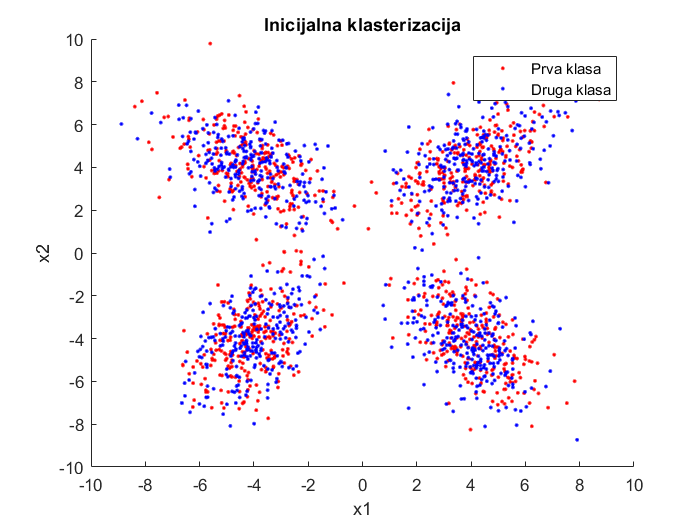
\includegraphics[width=1\textwidth]{pictures/4/CMean2Init}
\caption{Случај кад је $L=2$}\label{pic:cMean2Init}
\end{subfigure}
\begin{subfigure}{.55\textwidth}
\centering
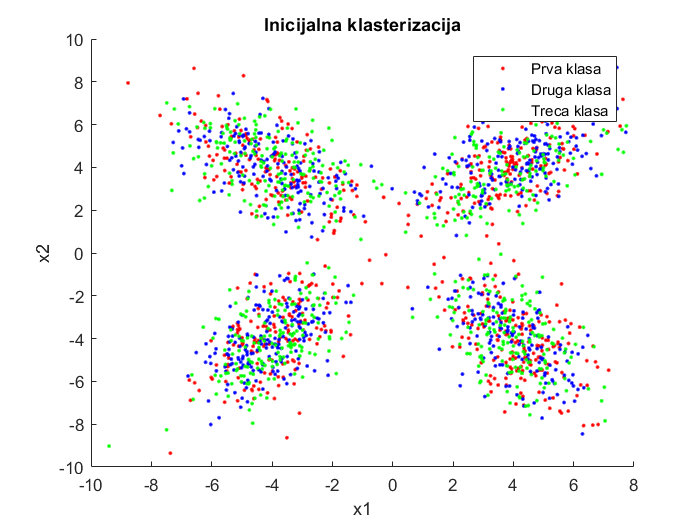
\includegraphics[width=1\linewidth]{pictures/4/CMean3Init}
\caption{Случај кад је $L=3$}\label{pic:cMean3Init}
\end{subfigure}
\bigskip
\begin{subfigure}{.55\textwidth}
\centering
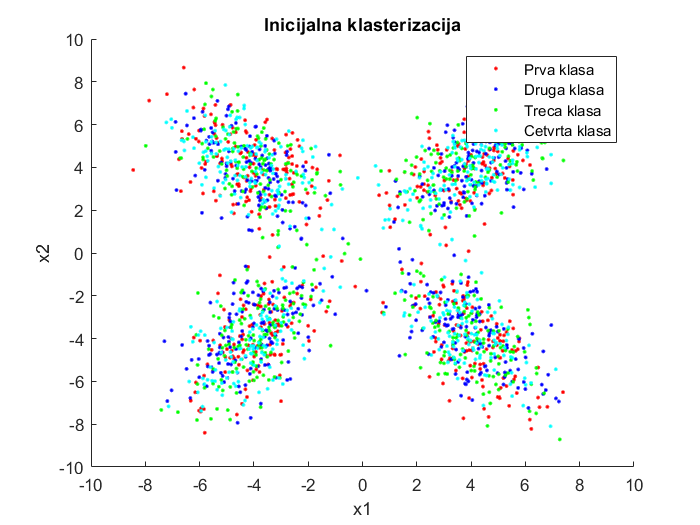
\includegraphics[width=1\linewidth]{pictures/4/CMean4Init}
\caption{Случај кад је $L=4$}\label{pic:cMean4Init}
\end{subfigure}
\begin{subfigure}{.55\textwidth}
\centering
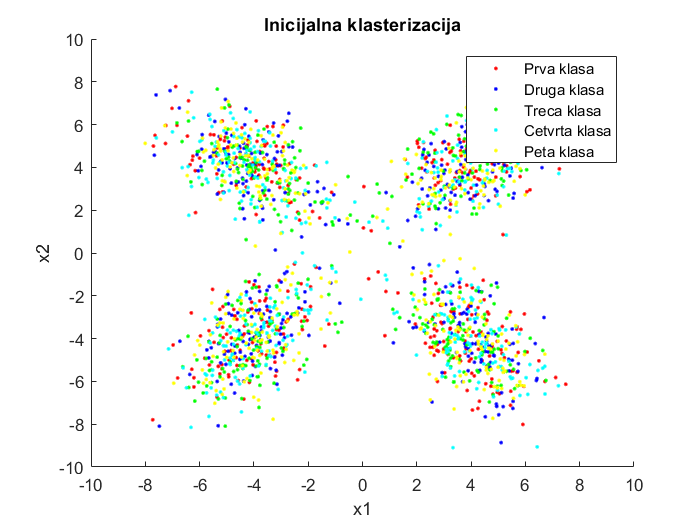
\includegraphics[width=1\linewidth]{pictures/4/CMean5Init}
\caption{Случај кад је $L=5$}\label{pic:cMean5Init}
\end{subfigure}
\end{figure}

Критеријум минимизује критеријумску функцију:
$$J=\frac{1}{N}\sum_{r=1}^L\sum_{j=1}^{N_r}||X_j^{(r)} - M_r||^2$$
где је $N$-укупан број одбирака, $L$-укупан број кластера, $M_r$-вектор средње вредности $r$-тог кластера, $N_r$-број елемената у $r$-том кластеру. С обзиром да критеријум минимизује средње квадратно одступање од центара кластера, закључује се да ће се сваки одбирак придружити најближем центру кластера. Међутим, овде се може закључити да C-mean узима у обзир само математичко очекивање, али не и коваријационе матрице одбирака. Сређивање израза добија се да је правило одлучивања:
$$||X_i - M_t(l)|| = \min_{1 \leq j \leq L}||X_i - M_j(l)|| \implies X_i \in \omega_t$$
Дакле прво се обави рекласификација, потом поново се израчуна $M_j(l)$ и то се извршава док има промене изгледа кластера. Кад нема завршава се.  Одсечци кода \ref{fun:cMeanClusterFind} и \ref{fun:cMeanCluster} су функције које имплементирају логику налажења минималне вредности критеријумске функције.

\begin{lstlisting}[caption={Функција налажења кластера за дате одбирке},label={fun:cMeanCluster}]
function [X1, X2, X3, X4, X5, changed] = reCluster(Y,M, curId)
changed = 0;
X1 = [];
X2 = [];
X3 = [];
X4 = [];
X5 = [];
 for i = 1 : size(Y, 1)
        clusterId = findClosesestDist(Y(i, :), M);
        if clusterId ~= curId
            changed = 1;
        end
        switch clusterId
            case 1
                X1 = [X1; Y(i, :)];
            case 2
                X2 = [X2; Y(i, :)];
             case 3
                X3 = [X3; Y(i, :)];
             case 4
                X4 = [X4; Y(i, :)];
            case 5
                X5 = [X5;  Y(i, :)];
        end
    end
end
\end{lstlisting}

\begin{lstlisting}[caption={Функција налажења кластера за дати одбирак},label={fun:cMeanClusterFind}]
function [clusterId] = findClosesestDist(elem, center)
for i = 1 : distLen
    curCenter = center(i, :);
    curDist = sqrt(sum((elem - curCenter).^2));
    if (curDist < distMin)
        distMin = curDist;
        distMinIdx = i;
    end
end
clusterId = distMinIdx;
\end{lstlisting}


Крајњи резултат извршавања се може видети на сликама  \ref{pic:cMean2Final}, \ref{pic:cMean3Final}, \ref{pic:cMean4Final}, \ref{pic:cMean5Final}.	

\begin{figure}[htb!]\caption{Крајња кластеризација}
\begin{subfigure}{.6\textwidth}
\centering
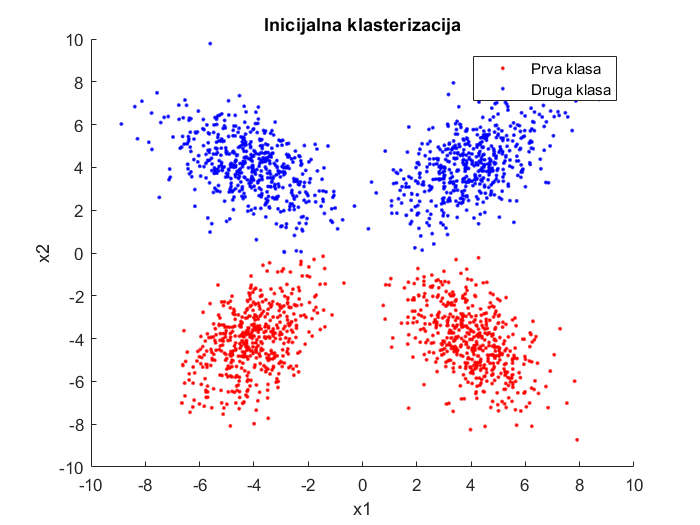
\includegraphics[width=1\textwidth]{pictures/4/CMean2Final}
\caption{Случај кад је $L=2$}\label{pic:cMean2Final}
\end{subfigure}
\begin{subfigure}{.55\textwidth}
\centering
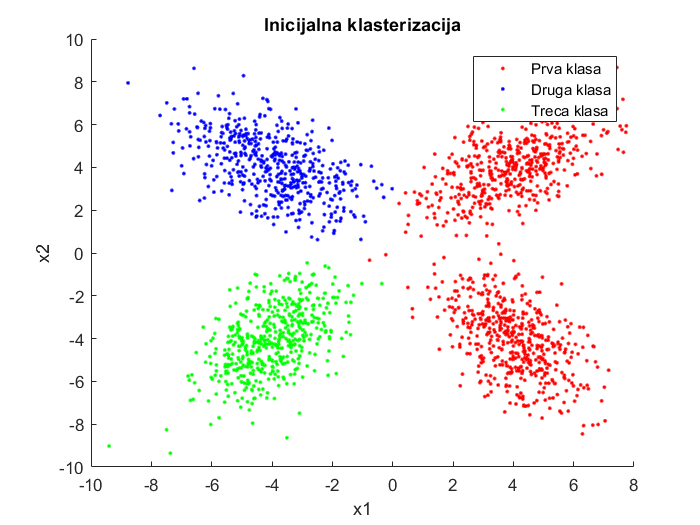
\includegraphics[width=1\linewidth]{pictures/4/CMean3Final}
\caption{Случај кад је $L=3$}\label{pic:cMean3Final}
\end{subfigure}
\bigskip
\begin{subfigure}{.55\textwidth}
\centering
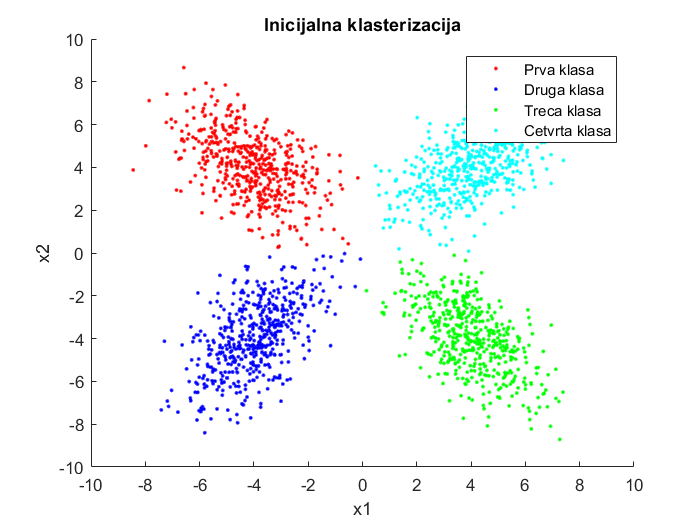
\includegraphics[width=1\linewidth]{pictures/4/CMean4Final}
\caption{Случај кад је $L=4$}\label{pic:cMean4Final}
\end{subfigure}
\begin{subfigure}{.55\textwidth}
\centering
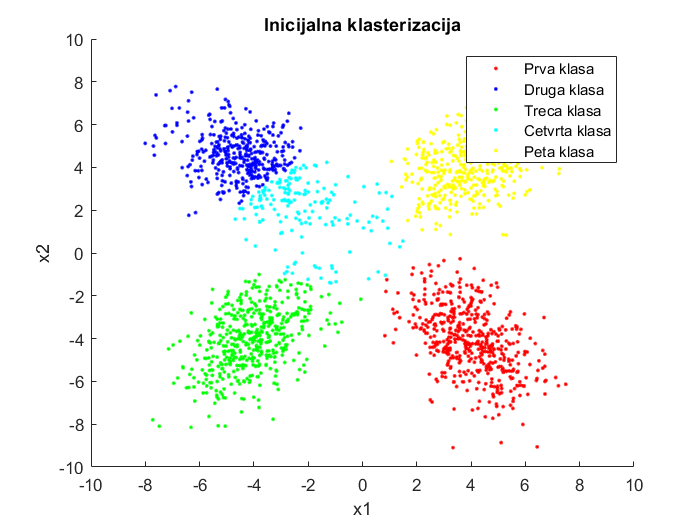
\includegraphics[width=1\linewidth]{pictures/4/CMean5Final}
\caption{Случај кад је $L=5$}\label{pic:cMean5Final}
\end{subfigure}
\end{figure}
\subsubsection{Анализа резултата алгоритма}
Алгоритам није превише осетљив на почетну кластеризацију, али не гарантује да ће се достићи оптимална кластеризација (у зависности од почетне расподеле у случају $L=4$ добије се изглед као \ref{pic:cMean3Final}). Просечан број итерација за иницијално претпостављене величине кластера $L=2, L=3, L=4,L=5$ варира, али усредњене вредности су редом $3,7 ; 5,93; 6,42; 9,13$. Ово је и у неку руку јасно јер су ове 4 класе на неки начин подељена на 2 скупа одбирака, односно 4, стога просечан број итерација расте драстично са случаја $L=2$ на случај $L=3$ и са $L=4$ на $L=5$, док са $L=3$ на $L=4$ не расте.  Ако је међутим познат број неких тачака које припадају одређеним кластерима, ово може да убрза рад алгоритма значајно. У случају $L=4$ добија се да за априорно вероватноћу познавања броја одбирака одређеног кластера $0,1$ просечан број одбирака је $3,7$ а за случај $0,25$ спада на 3, а за $0,5$ чак je спао на $2,3$, што је и логично јер су кластери већ у неку руку одређени. 

Уколико априорно није познат број кластера неопходно је одрадит минимизацију коришћењем неког критеријума. Мало измењена верзија Акаикевог критеријума $AIC(L) =J(L) + ln(L)$ где је $J(L)$ минимизирана критеријумска функција за конкретан број кластера. Редом, за различит број класа 2, 3, 4, 5 су добијене $20, 10;12.8;5,194;5,68$.  Што и каже оно што видимо на слици, да постоје 4 класе.

\subsection{Метод квадратне декомпозиције}
\subsubsection{Генерисање одбирака}
За почетак генерисаћемо одбирке двеју дводимензионалних класа чије су функције густине вероватноће у облику бимодалних гаусовских расподела:


$$f_1(X) = P_{11} N(M_{11}, \Sigma_{11}) + P_{12} N(M_{12}, \Sigma_{12})$$
$$f_2(X) = P_{21} N(M_{21}, \Sigma_{21}) + P_{22} N(M_{22}, \Sigma_{22}),$$
при чему вероватноће, средње вредности и коваријационе матрице имају следеће вредности:
$$P_{11} = 0,6,  M_{11} = \begin{bmatrix}
   1,5\\
   -4,5
\end{bmatrix}, 
S_{11} = \begin{bmatrix}
				   3,5 & -1\\
				   -1 & 2,2
				\end{bmatrix},
P_{12} = 0,4,  M_{12} = \begin{bmatrix}
										   -0,5\\
										   0,5
										\end{bmatrix}, 
S_{12} = \begin{bmatrix}
				   1,3 & 0,9\\
			   	0,9 &  2
				\end{bmatrix}
$$				
$$P_{21} = 0,45,  M_{21} = \begin{bmatrix}
   12\\
   -3,5
\end{bmatrix}, 
S_{21} = \begin{bmatrix}
				   1,5 & 1,1\\
				   1,1 & 1,5
				\end{bmatrix},
P_{22} = 0,55,  M_{22} = \begin{bmatrix}
										   -10\\
										   2
										\end{bmatrix}, 
S_{22} = \begin{bmatrix}
				   3 & -0,8\\
			   	-0,8 &  3
				\end{bmatrix}
$$

Добијају се 2 класе одбирака као на слици \ref{fig:OdbirciQuad}.

\begin{figure}[htb!]
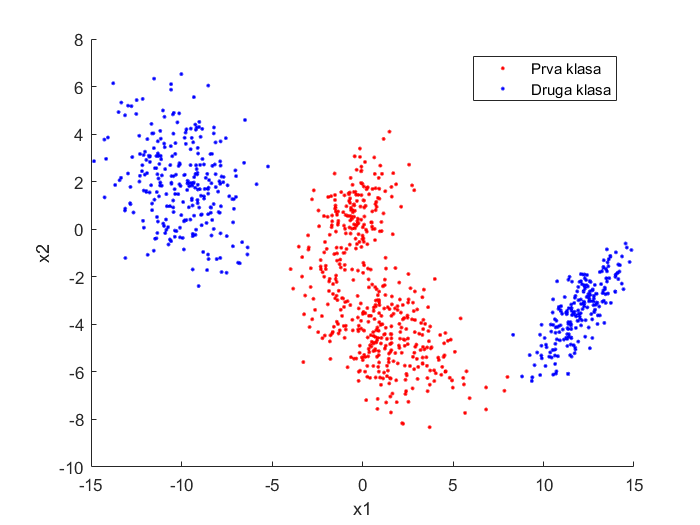
\includegraphics[scale=.8]{pictures/4/OdbirciQuad}
\caption{Одбирци}\label{fig:OdbirciQuad}
\end{figure}

\subsubsection{Алгоритам}
Овај метод је сложенији и захтевнији за израчунавање. Али његова предност је што границе изђему кластера не морају да буду само линеарне, него су квадратне криве. Стога се он употребљава кад је потребна кластеризација нелинеарлно сепарабилних класа. 
Одсечак кода представља \ref{fun:quadr} имплементацију алгоритма.

На почетку се изабере иницијална кластеризација $\Omega(0)$ И на основу ње процене априорне вероватноће појава $P_i(0)$ вектори средњих вредности класа $M_i(0)$, Као и коваријационе матриц $\Sigma_i(0)$. У свакој итерацији одбирак $X_j$ се придрућује класи $t$ за коју је дати израз најмањи:
$$(X_j - M_t(l))^T\Sigma_t^{-1}(l)(X_j-M_t(l)) + ln|\Sigma_t(l)| - ln(P_t(l))$$
Логика испитивања минималне вредност критеријумске функције имплементирана је функцијом чији је одсечак кода је  \ref{fun:reclusterQuadr} и функцијом чији одсечак кода је \ref{fun:reclusterQuadSearch} .

\begin{lstlisting}[caption={Метод квадратне декомпозиције},label={fun:quadr}]
function [num_it, critFun] = quadratic(X1, X2, num_points, num_classes, apPer, drawFigure)

chunkRand = floor((1 - apPer) * num_points);
chunkApp = num_points - chunkRand;

Z = [X1(1 : chunkRand, :); X2(1 : chunkRand, :);];

num_points_all = 2 * chunkRand;

idx = randperm(num_points_all);
chunk_size = floor(num_points_all / num_classes);

Y1 = Z(idx(1 : chunk_size), :);
Y1App = X1(chunkRand + 1 : num_points, :);
Y1 = [Y1App; Y1];
Y2 = Z(idx(chunk_size + 1:2 * chunk_size), :);
Y2App = X2(chunkRand + 1 : num_points, :);
Y2 = [Y2App; Y2];
Y3 = [];
Y3App = [];
Y4 =[];
Y4App = [];
Y5 =[];
Y5App = [];
if (num_classes > 2)
    Y3 = Z(idx(2 * chunk_size + 1:3 * chunk_size), :);
end 
if (num_classes > 3)
    Y4 = Z(idx(3 * chunk_size + 1:4 * chunk_size), :);
end
if (num_classes > 4)
    Y5 = Z(idx(4 * chunk_size + 1:5 * chunk_size), :);
end

run = 1;

it = 0;

while (run && it < 50)
    it = it + 1;
    M1 = mean(Y1);
    M2 = mean(Y2);
    M3 = mean(Y3);
    M4 = mean(Y4);
    M5 = mean(Y5);
    
    S1 = cov(Y1);
    S2 = cov(Y2);
    S3 = cov(Y3);
    S4 = cov(Y4);
    S5 = cov(Y5);
    P1 = size(Y1, 1) / (2 * num_points);
    P2 = size(Y2, 1) / (2 * num_points);
    P3 = size(Y3, 1) / (2 * num_points);
    P4 = size(Y4, 1) / (2 * num_points);
    P5 = size(Y5, 1) / (2 * num_points);
    
    if (size(M1, 2) == 1)
        M1 = [realmax realmax];
        S1 = [realmax realmax; realmax realmax];
    end 
    if (size(M2, 2) == 1)
        M2 = [realmax realmax];
        S2 = [realmax realmax; realmax realmax];
    end 
    if (size(M3, 2) == 1)
        M3 = [realmax realmax];
        S3 = [realmax realmax; realmax realmax];
    end 
    if (size(M4, 2) == 1)
        M4 = [realmax realmax];
        S4 = [realmax realmax; realmax realmax];
    end 
    if (size(M5, 2) == 1)
        M5 = [realmax realmax];
        S5 = [realmax realmax; realmax realmax];
    end 
    clear X1 X2 X3 X4;
    
    M = [M1; M2; M3; M4; M5];
    S = [S1; S2; S3; S4; S5];
    P = [P1; P2; P3; P4; P5];
    
    [X11, X21, X31, X41, X51, changed1] = reClusterQuadr(Y1(chunkApp + 1: end, :), M, S, P, 1);
    [X12, X22, X32, X42, X52, changed2] = reClusterQuadr(Y2(chunkApp + 1: end, :), M, S, P, 2);
    [X13, X23, X33, X43, X53, changed3] = reClusterQuadr(Y3(chunkApp + 1: end, :), M, S, P, 3);
    [X14, X24, X34, X44, X54, changed4] = reClusterQuadr(Y4(chunkApp + 1: end, :), M, S, P, 4);
    [X15, X25, X35, X45, X55, changed5] = reClusterQuadr(Y5(chunkApp + 1: end, :), M, S, P, 5);
    run = changed1 | changed2 | changed3 | changed4 | changed5;
    Y1 = [Y1App; X11; X12; X13; X14; X15];
    Y2 = [Y2App; X21; X22; X23; X24; X25];
    Y3 = [Y3App; X31; X32; X33; X34; X35];
    Y4 = [Y4App; X41; X42; X43; X44; X45];
    Y5 = [Y5App; X51; X52; X53; X54; X55];
end

num_it = it;
\end{lstlisting}

\begin{lstlisting}[caption={Функција проналажења одговарајућег кластера},label={fun:reclusterQuadr}]
function [X1, X2, X3, X4, X5, changed] = reClusterQuadr(Y, M, S, P, curId)
changed = 0;
X1 = [];
X2 = [];
X3 = [];
X4 = [];
X5 = [];
 for i = 1 : size(Y, 1)
        clusterId = findClosesestDistQuadr(Y(i, :), M, S, P);
        if clusterId ~= curId
            changed = 1;
        end
        switch clusterId
            case 1
                X1 = [X1; Y(i, :)];
            case 2
                X2 = [X2; Y(i, :)];
             case 3
                X3 = [X3; Y(i, :)];
             case 4
                X4 = [X4; Y(i, :)];
            case 5
                X5 = [X5;  Y(i, :)];
        end
    end
end
\end{lstlisting}

\begin{lstlisting}[caption={Функција проналажења одговарајућег кластера},label={fun:reclusterQuadSearch}]
function [clusterId] = findClosesestDistQuadr(elem, M, S, P)
distLen = size(M, 1);
distMinIdx = 0;
distMin = realmax;
for i = 1 : distLen
    curM = M(i, :);
    curS = S(2 * i - 1 : 2 * i, :);
    curP = P(i, :);
    if (S(2*i - 1, 1) > 10000)
        j = realmax;
    else
        j = (elem - curM) * inv(curS) * (elem - curM)' + log(det(curS)) - log(curP);
    end
    if (j < distMin)
        distMin = j;
        distMinIdx = i;
    end
end
clusterId = distMinIdx;
\end{lstlisting}

 На почетку алгоритма имамо насумично кластеризовање података.  На сликама  \ref{pic:Quad2Init}, \ref{pic:Quad3Init}, \ref{pic:Quad4Init}, \ref{pic:Quad5Init} видимо почетне кластеризације за различит број почетних класа. 
\begin{figure}[htb!]\caption{Иницијална кластеризација}
\begin{subfigure}{.6\textwidth}
\centering
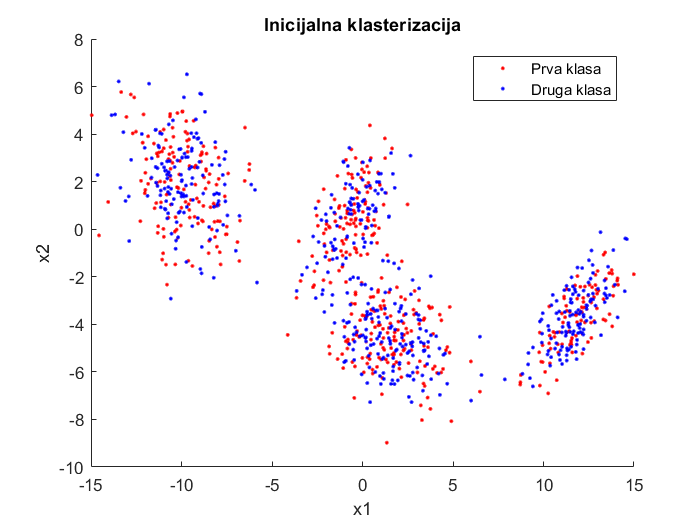
\includegraphics[width=1\textwidth]{pictures/4/Quad2Init}
\caption{Случај кад је $L=2$}\label{pic:Quad2Init}
\end{subfigure}
\begin{subfigure}{.55\textwidth}
\centering
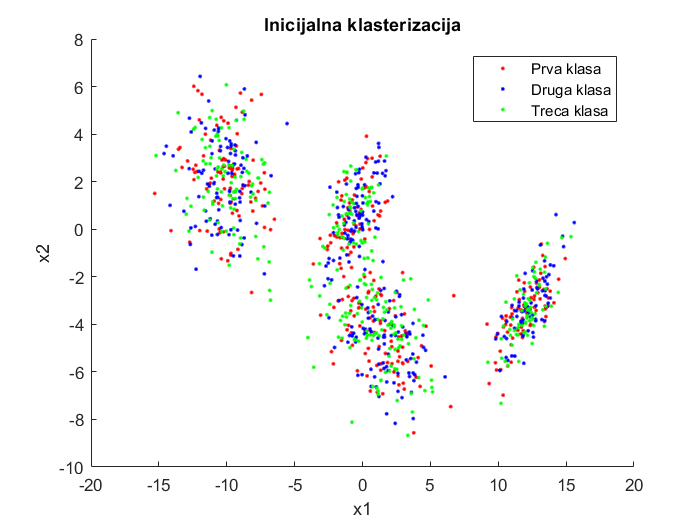
\includegraphics[width=1\linewidth]{pictures/4/Quad3Init}
\caption{Случај кад је $L=3$}\label{pic:Quad3Init}
\end{subfigure}
\bigskip
\begin{subfigure}{.55\textwidth}
\centering
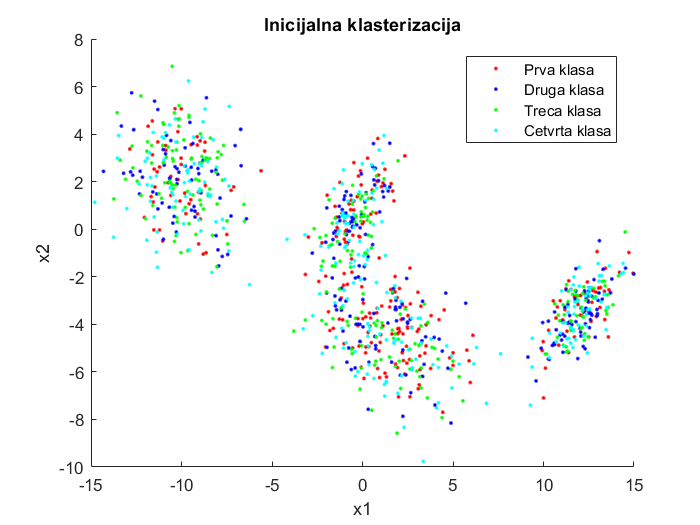
\includegraphics[width=1\linewidth]{pictures/4/Quad4Init}
\caption{Случај кад је $L=4$}\label{pic:Quad4Init}
\end{subfigure}
\begin{subfigure}{.55\textwidth}
\centering
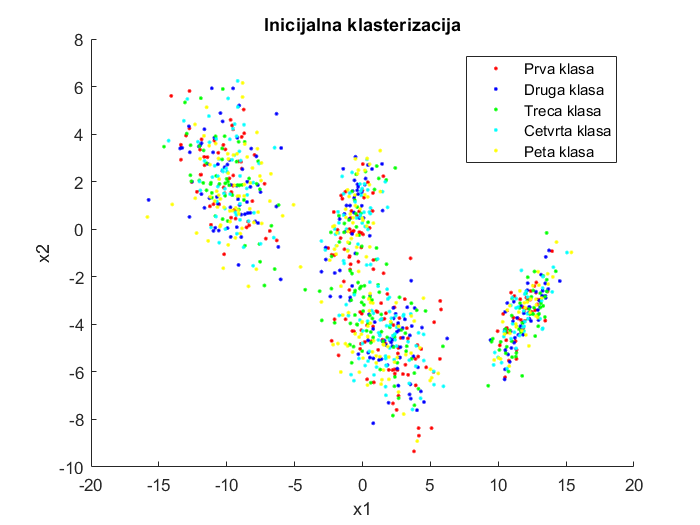
\includegraphics[width=1\linewidth]{pictures/4/Quad5Init}
\caption{Случај кад је $L=5$}\label{pic:Quad5Init}
\end{subfigure}
\end{figure}

Крајњи резултат извршавања се може видети на сликама  \ref{pic:Quad2Final}, \ref{pic:Quad3Final}, \ref{pic:Quad4Final}, \ref{pic:Quad5Final}.	 Дакле алгоритам уопште не кластеризује добро.
\begin{figure}[htb!]\caption{Крајња кластеризација}
\begin{subfigure}{.6\textwidth}
\centering
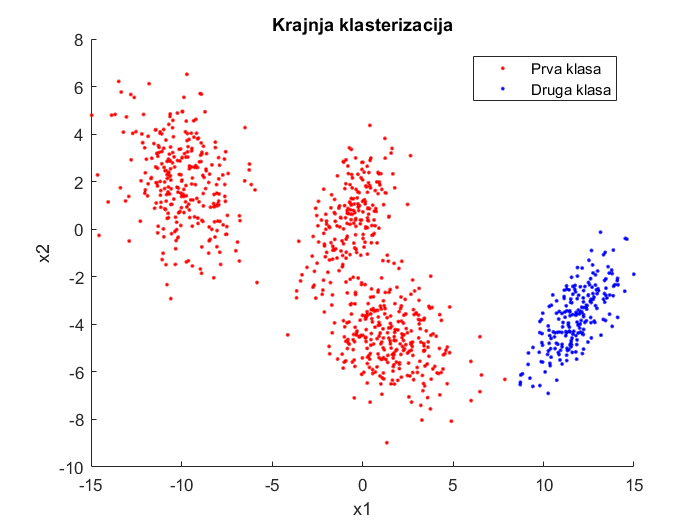
\includegraphics[width=1\textwidth]{pictures/4/Quad2Final}
\caption{Случај кад је $L=2$}\label{pic:Quad2Final}
\end{subfigure}
\begin{subfigure}{.55\textwidth}
\centering
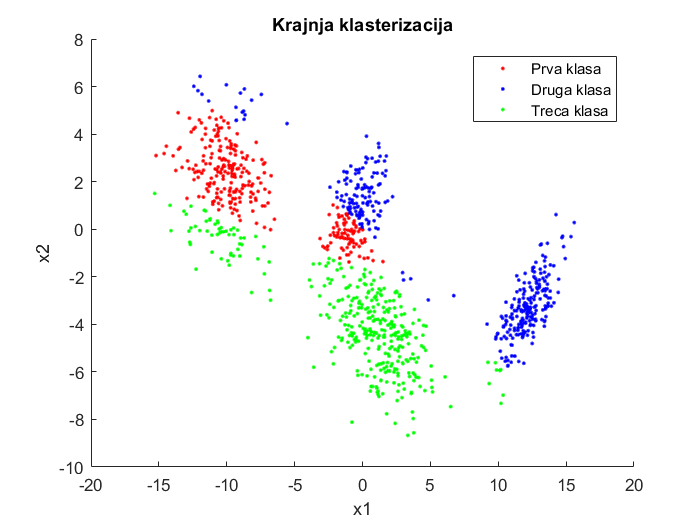
\includegraphics[width=1\linewidth]{pictures/4/Quad3Final}
\caption{Случај кад је $L=3$}\label{pic:Quad3Final}
\end{subfigure}
\bigskip
\begin{subfigure}{.55\textwidth}
\centering
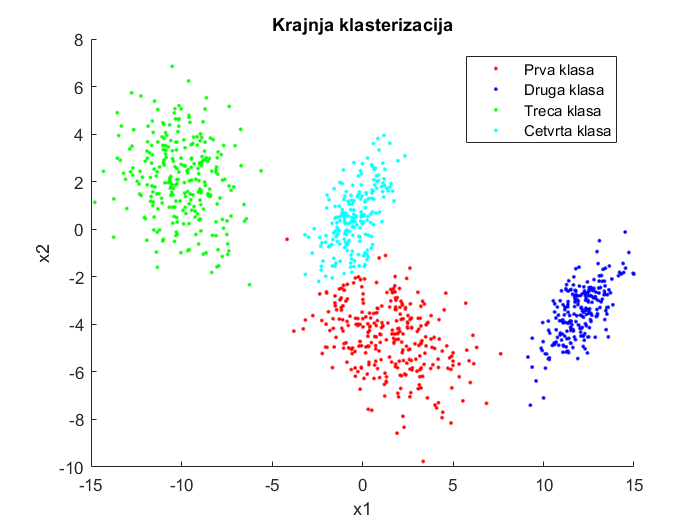
\includegraphics[width=1\linewidth]{pictures/4/Quad4Final}
\caption{Случај кад је $L=4$}\label{pic:Quad4Final}
\end{subfigure}
\begin{subfigure}{.55\textwidth}
\centering
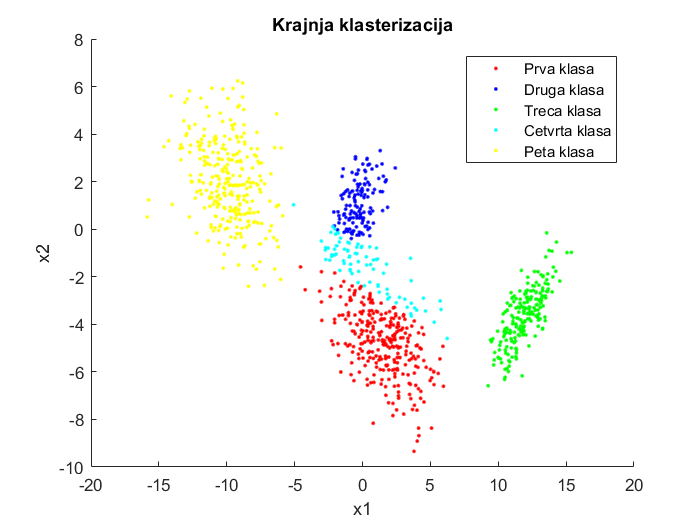
\includegraphics[width=1\linewidth]{pictures/4/Quad5Final}
\caption{Случај кад је $L=5$}\label{pic:Quad5Final}
\end{subfigure}
\end{figure}


\subsubsection{Анализа резултата}
Алгоритам је осетљив на почетну кластеризацију, и не гарантује да ће се достићи оптимална кластеризација. Просечан број итерација за иницијално претпостављене величине кластера $L=2, L=3, L=4,L=5$ варира, али усредњене вредности су редом $10.2 ; 17.9; 20.4; 20.1$. Ово је и у неку руку јасно јер су ове 2 класе на неки начин подељена на 2 скупа одбирака, стога просечан број итерација расте драстично са случаја $L=2$ на случај $L=3$ и релативно,  драстично са $L=3$ на $L=4$ док са $L=4$ на $L=5$ чак и опада.  Ако је међутим познат број неких тачака које припадају одређеним кластерима, ово може да убрза рад алгоритма значајно и да се постигне тачност. У случају $L=4$ добија се да за априорно вероватноћу познавања броја одбирака одређеног кластера $0,1$ просечан број одбирака је $7,1$ а за случај $0,25$ спада на $6$а за $0,5$ чак je спао на $4,6$. Такође, са порастом априорне вероватноће познавања броја одбирака одређеног кластера, добија се пуно већа тачност, што за вероватноће $0,15$ и $0,25$ можемо да видимо на сликама \ref{pic:Quad15Final} и \ref{pic:Quad20Final} да је релативно добро одредио кластере.

Уколико априорно није познат број кластера неопходно је одрадит минимизацију коришћењем неког критеријума. Мало измењена верзија Акаикевог критеријума $AIC(L) =J(L) +3 ln(L)$ где је $J(L)$ минимизирана критеријумска функција за конкретан број кластера. Редом, за различит број класа 2, 3, 4, 5 су добијене $8,778;8,76;8,62;9,16$.  Што и каже оно што видимо на слици, да постоје 2 класе, али подједнаке шансе постоје и да постоје 3 и 4.

\begin{figure}[htb!]\caption{Крајња кластеризација}
\begin{subfigure}{.6\textwidth}
\centering
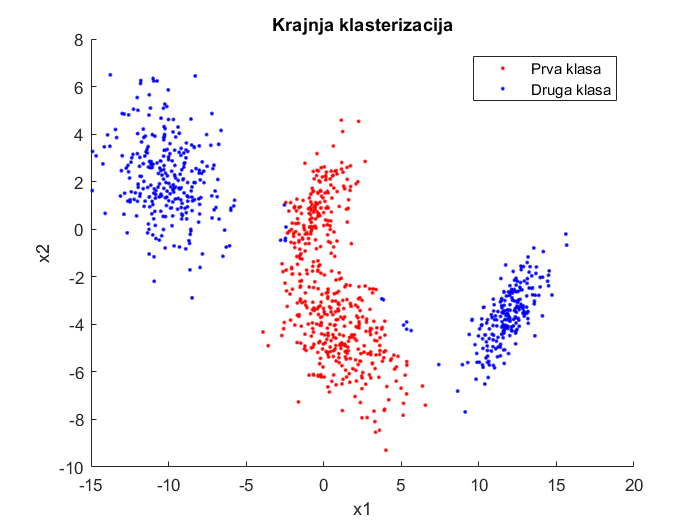
\includegraphics[width=1\textwidth]{pictures/4/QuadrFinal15}
\caption{Случај кад је априорна вероватноћа 15\%}\label{pic:Quad15Final}
\end{subfigure}
\begin{subfigure}{.55\textwidth}
\centering
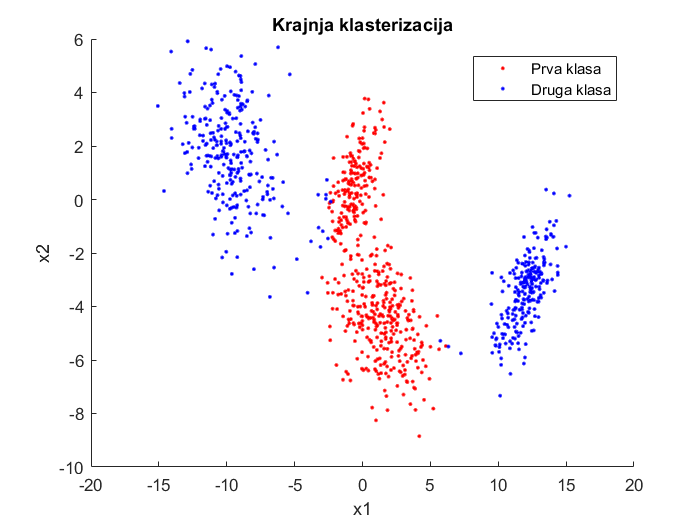
\includegraphics[width=1\linewidth]{pictures/4/QuadrFinal25}
\caption{Случај кад је априорна вероватноћа 25\%}\label{pic:Quad20Final}
\end{subfigure}

\end{figure}










\end{document}
